% \documentclass[linenumbers,summarypage,hyperlinks]{outhesis}
\documentclass{outhesis}

% For a bibliography style, you must have the appropriate .bst file
% \bibliographystyle{apj}
\bibliographystyle{prsty}

% Provide the correct margins
\usepackage[top=1in, bottom=1in, left=1.6in, right=1.2in]{geometry}
% If you want a double-sided copy for yourself, uncomment the next line
 % \usepackage[twoside,top=1in, bottom=1in, left=1.6in, right=1.2in]{geometry}

\usepackage{hepparticles}
\usepackage{indentfirst}
\usepackage{subfigure}
\usepackage[makeroom]{cancel}
\usepackage{float}
\usepackage{setspace}

\begin{document}

%% Place Dissertation information here
%% Follow the convention for the use of capital letters 
%% or else the font will not be formatted properly
\author{Othmane Rifki}
\university{UNIVERSITY OF OKLAHOMA}
\college{GRADUATE COLLEGE}
\department{HOMER L. DODGE DEPARTMENT OF PHYSICS AND ASTRONOMY}
\title{THE MUON ANOMALOUS MAGNETIC MOMENT:\\ A PROBE FOR THE STANDARD MODEL AND BEYOND}
\address{Norman, Oklahoma}
\yr{2014}
\dgname{SPECIALIST'S EXAMINATION}
%% List your committee members here
\committee{{Dr. Brad Abbott, Chair}, {Dr. S. Lakshmivarahan, Outside Member}, Dr. Mike Strauss, Dr. Chung Kao, Dr. Eric Abraham}

%% Put your dedication here. This is completely optional. Delete it if you don't need it.
%\begin{dedication}
 % 
%\end{dedication}

%% Put your acknowledgements here. This is completely optional. Delete it if you don't need it.
%\begin{acknowledgements}
%  
% \end{acknowledgements}

%% Put your abstract here.

\begin{abstract}
\singlespacing

The muon is a spin-$\frac{1}{2}$ charged particle characterized by an intrinsic magnetic moment with a gyromagnetic ratio, $g$, that is very close to 2. Its variance from 2, referred to as the magnetic moment anomaly $\displaystyle a_{\mu} = \frac{g-2}{2}$, has been determined over the last decades to ever higher precisions in both experiment and theory. The most recent experiment (E821) was performed at Brookhaven National Laboratory and achieved a precision of 0.54 ppm, while the current theoretical evaluation stands at a precision of 0.39 ppm. However, the experimental value is higher than the predicted value by more than 3 standard deviations which suggests the possibility of new physics. A new experiment (E989) is being constructed at Fermi National Laboratory to investigate the discrepancy by reducing the experimental error to 0.14 ppm. At the same time, theory groups are working to reduce the error in $a_{\mu}$ to match the projected experimental precision. A confirmation of the difference between experiment and theory will have an impact on new physics models in the TeV scale. The goal of this review is to describe the E821 measurement of $a_{\mu}$, the improvements implemented in E989, the current theoretical status in the computation of $a_{\mu}$, and the new physics implications.

\end{abstract}


\frontmatter

\maketitle

\mainmatter
\singlespacing


\noindent{ \emph{The closer you look the more there is to see.}} \\
\indent{Friedrich Jegerlehner, \emph{The Anomalous Magnetic Moment of the Muon} \cite{book}.}



\section{Introduction}
\label{sec:intro}

The study of elementary particles and their interactions led to a representative mathematical formulation known as the \emph{Standard Model} (SM) of particle physics. When subjected to experimental tests, the SM successfully describes three of the four fundamental forces: electromagnetic, weak, and strong interactions. On the other hand, the SM is not believed to be complete since it fails to explain a number of problems that are still facing today's physics community. First, the SM does not incorporate the fourth fundamental force of gravity. Moreover, It does not provide insight on the nature of the ``invisible'' matter that is holding galaxies together, which constitutes $\sim$ 26\% of the energy density of the universe and is known as \emph{Dark Matter}. In addition, the SM does not account for the different masses and mixing of the 12 leptons
 known as the \emph{flavor problem}, and the predominance of matter over antimatter. In order to solve these problems, searches for physics not accounted for by the SM have been pursued in both experiment and theory. Any sign of significant discrepancy between experiment and theory is taken very seriously since it might lead to new insights that can reveal what is missing in our current view of the universe. Some physicists have set up experiments to look for answers to SM problems by studying high energy interactions as is pursued at the Large Hadron Collider at CERN, in the hope of observing some new particles. This led to the discovery of the Higgs boson in 2012, a central piece of the SM. Other experiments have been set up to perform detailed studies of known particles, measuring their properties to very high precisions and comparing them to theoretical calculations to both check the models and look for discrepancies. The subject of this current review is an important illustration of the latter scenario where precision tests of the
\emph{magnetic moment}, an intrinsic property of a spinning charged elementary particle, will be examined by comparing experiment to theory.

The possible elementary charged particles that can be used to measure the magnetic moment are the three spin $\frac{1}{2}$ leptons: the electron $e$, the muon $\mu$, and the tau $\tau$. While these particles have the same charge and spin, they have very different masses\footnote{The unit of mass is given in MeV/c$^2$ according to the relation $E = m c^2$ with the energy $E$ given in units of MeV where 1 MeV = 1.6 $\times$ 10$^{-13}$J.} which are given by $m_e$ = 0.511 MeV$/c^2$, $m_{\mu}$ = 105.658 MeV$/c^2$, and $m_{\tau}$ = 1776.82 MeV$/c^2$. The difference in masses alters the lifetimes and decay modes of each particle. The electron is the lowest mass charged lepton and thus is stable. The muon lifetime is $\tau_{\mu} = 2.197 \times 10^{-6}$ seconds and it decays almost 100\% to an electron and two neutrinos ($e\nu_{\mu}\bar{\nu_{e}}$). Taus have a much shorter lifetime $\tau_{\tau} = 2.906 \times 10^{-13}$ seconds and a diversified decay pattern where 65\% go into hadronic states (states that contain quark-antiquark pair particles such as pions) and the remainder go into leptonic states (the two possible states are muons and two neutrinos or electrons and two neutrinos) \cite{pdg}. Because of its very short lifetime, the study of the tau's magnetic moment is 
difficult, leaving the electron and the muon as the practical candidates for measuring the magnetic moment. While the electron is the most precisely studied lepton, effects in the magnetic moment sensitive to physics beyond the SM scale with powers of $m_\ell^2$
\cite{phen}. For this reason, muons are more appropriate for the study of the magnetic moment to search for new physics. 
The magnetic moment arises from the electric charge and the current of an elementary particle with spin. For instance, a classical calculation of a particle with mass m, and charge q, moving in a circular orbit of radius $r$, with velocity $\overrightarrow{v}$, shows that its magnetic moment $\overrightarrow{\mu}$ is related to its orbital angular momentum ($\overrightarrow{L} =m\overrightarrow{r} \times \overrightarrow{v}$) by the relation: 
\begin{equation}
\overrightarrow{\mu} = \frac{q}{2mc} \overrightarrow{L}.
  \label{eq:L}
\end{equation}

In quantum mechanics, the magnetic moment is an intrinsic property of a particle with spin. Both the magnetic moment and the orbital angular momentum are promoted to operators in order to give the correct quantum mechanical representation. While Equation (\ref{eq:L}) is still valid in describing the orbital angular momentum $\overrightarrow{L}$, the spin magnetic moment requires a modification by a factor $g$ that is very close to 2. The corrected equation is given by
\begin{equation}
\overrightarrow{\mu} = g\frac{q}{2mc}\overrightarrow{S},
\label{eq:mu}
\end{equation}
where $g$ is called the \emph{gyromagnetic ratio}, the \emph{Lande g-factor}, or the  \emph{g-factor}, and $q$ is the charge given in units of the fundamental charge $e$, where $q = -e$ for a lepton particle (negative muon) and $q = +e$ for a lepton antiparticle (positive muon). $\overrightarrow{S}$ is the spin operator
\begin{equation}
\overrightarrow{S} = \frac{\hbar}{2}\overrightarrow{\sigma},
\end{equation} 
where $\sigma_i$ are the Pauli spin matrices. 
The result $g = 2$ was first obtained by Dirac in 1928 when he generalized the Schr\"{o}dinger equation to incorporate special relativity (See Appendix \ref{app:dirac}). With the development of the quantum mechanical description of electromagnetism known as quantum electrodynamics (QED), $g$ was found to differ from 2 by an anomaly $a_\ell$, known as the  \emph{magnetic moment anomaly}, or the \emph{anomaly} for short, such that: $g_\ell = 2(1+a_\ell)$. The anomaly is then
\begin{equation}
a_{\ell} = \frac{g_\ell-2}{2}.
\end{equation}
In this equation, the $g-2$ factor appears! The factor $g-2$ is incorporated in the title of all experiments that measure the magnetic moment of the muon and it is the focus of this review.

In addition to the quantum fluctuations of the electromagnetic field described by QED, quantum fluctuations due to heavier particles such as the weak gauge bosons (W$^{\pm}$ and Z bosons) and hadrons (for example quark-antiquark pairs such as pions) also contribute to the anomaly. These effects are known as radiative corrections (RC) and are mainly dominated by QED as it will be discussed in Section \ref{sec:sm}. The anomaly scales as $\delta a_\ell \sim \frac{m_\ell^2}{M^2}$  where $M\gg m_\ell$ can represent the mass of a heavier SM particle, the mass of an unobserved heavy particle beyond the SM, or an energy range where the SM is no longer valid \cite{phen}. From this relation, we first see that $a_{\mu}$ is more sensitive to new effects than $a_e$ by a factor of $\left(m_{\mu}/m_e\right)^2 \approx 4 \times 10^4$. On the other hand, heavier states (large M) have smaller effects ($\sim 1/M^2$) which places the determination of $g-2$ as a good probe for interactions with energies at the TeV scale. The LHC is currently probing the TeV energy scale, so $g-2$ will complement and guide the LHC searches and may even be more sensitive to new physics that is not accessible to the LHC. 

The importance of $g-2$ is in the fact that it can be precisely measured, as it will be discussed in Section \ref{sec:exp} and it can be precisely calculated based on all RC of the SM as will be discussed in Section \ref{sec:sm}. 
On the experimental side, the most recent experiment is the Brookhaven National Laboratory (BNL) E821 $g-2$ experiment that concluded its run in 2001, with a final reported result of \cite{bnl}:
\begin{equation}
a_{\mu}^{\text{E821}} = \left(116\, 592\, 08.0 \pm 6.3\right) \times 10^{-10} \left(0.54  \text{ ppm}\right) \cite{bnl},
\label{eq:exp}
\end{equation}
where ppm refers to the precision in parts per million given by the ratio of the total error to the value as $\sigma_X/X$. 
The anomaly has been evaluated by different groups. One of its recent calculations is
\begin{equation}
a_{\mu}^{SM} = \left(116\, 591\, 82.8 \pm 4.5\right) \times 10^{-10} \left(0.39  \text{ ppm}\right)  \,\,\cite{hadlo2},
\label{eq:sm}
\end{equation}
which gives a difference of 
\begin{equation}
\Delta a_{\mu} \left(\text{E821} - \text{SM} \right) = \left(25.2 \pm 7.7\right) \times 10^{-10}.  
\label{eq:diff}
\end{equation}
The difference $\Delta a_{\mu}$ between the measurement and the prediction is 3.3 standard deviations with the measurement having the higher value. In particle physics, a three standard deviation effect ``$3\sigma$" means that the probability of the measurement to randomly fluctuate from the predicted value by $3\sigma$ is equivalent to the probability of obtaining a value on a Gaussian distribution that is at least 3 standard deviations away from the expected mean. This corresponds to a probability of $1.35 \times 10^{-3}$ (on average 1 out of every 740 measurements). In order to be confident that the difference is not just a statistical fluctuation, a difference of five standard deviations ``$5\sigma$" is required, which implies that the probability of such variation is $3 \times 10^{-7}$ (on average 1 out of every 3.5 million measurements).  

An independent experiment is designed to reduce the error in Equation (\ref{eq:exp}) to $\sim 1.6 \times 10^{-10}$ giving a precision of 0.14 ppm with a four-fold improvement over the BNL result \cite{bnl}.
%sqrt(1.6^2+4.9^2)=5.15, 27.8/5.15 = 5.4  same for the other.
Assuming that a similar value for the anomaly is obtained and the theoretical calculation is exactly the same, the new deviation is $5.3\sigma$, which will confirm the discrepancy. This new experiment is currently being built at Fermi National Laboratory (FNAL) under the name E989 Muon $g-2$ Experiment. An error improvement in the measurement of $g-2$ implies that the error in the calculated prediction should also be improved to the same level.
In the event that E989 confirms this discrepancy, severe constraints will be imposed on new theoretical models such as supersymmetry,\footnote{Supersymmetry (SUSY) theory postulates that a space-time symmetry exists between the two classes of the SM elementary particles: fermions and boson. It incorporates the four fundamental forces and predicts energy interactions beyond the weak scale. However, experimental evidence has yet to support the theory.} extra dimensions,\footnote{Extra dimension models postulate the existence of dimensions other than the three spatial dimensions and the temporal dimension.} or a dark matter particle. 

This review will describe the experimental technique used to measure the anomaly and present the status of the theoretical calculations. It will also address the future improvements in both areas and conclude with new physics possibilities.


\section{Properties of the Muon}


The muon anomaly can be measured to ppm precision by studying the behavior of the spin magnetic moment of muons in circular orbits subjected to a uniform magnetic field. In this section, the key ideas that permit the measurement will be introduced to lead up to a discussion of the BNL experiment in the next section. 



\subsection{Obtaining Polarized Muons}

Muons are obtained from pions that are acquired from sending a high intensity beam of protons into a target material that has the property of being resistant to high stresses, \emph{nickel} for example. The decay of positive and negative pions produces positive and negative muons according to 
\begin{equation}
\begin{split}
&\pi^+ \rightarrow \HepParticle{\mu}{}{+} +\HepParticle{\nu}{\mu}{},\\
&\pi^- \rightarrow \mu^- + \HepAntiParticle{\nu}{\mu}{}.
\end{split}
\end{equation}
The spin orientation, called \emph{polarization},  of the decayed muon is well determined for the cases of positive and negative pions. This can be seen by introducing the concepts of \emph{helicity}, \emph{parity transformation}, and \emph{charge conjugation}. Helicity is defined as the projection of spin $\overrightarrow{S}$ along the momentum direction $\hat{p} = \overrightarrow{p}/|\overrightarrow{p}|$ such that $h = \overrightarrow{S}\cdot \hat{p}$. For a spin-$\frac{1}{2}$ particle, it is right-handed when $h=+1/2$ (spin and momentum parallel) and left-handed when $h=-1/2$ (spin and momentum anti-parallel). Parity, represented by the operator $P$, creates the mirror image of a physical process. For example, for a vector $\overrightarrow{x}$, $P\ket{\overrightarrow{x}} = -\ket{\overrightarrow{x}}$. Charge conjugation, represented by the operator $C$, refers to the conversion of a particle to its antiparticle by changing the sign of all its quantum numbers (electric charge, lepton number, baryon number, and flavor charges such as strangeness). 

By starting from a spin zero pion and a right-handed antineutrino, the possible transformations are $C$, $P$, or both $CP$ as shown in Figure \ref{fig:cp}. Experimental evidence shows that neutrinos can only be left-handed and antineutrinos can only be right-handed. For this reason, the only possible process is the one obtained by a CP transformation, which makes a negative pion produce a right-handed negative muon ($h=+1/2$), and a positive pion produce a left-handed positive muon ($h=-1/2$). 
\begin{figure}
  \centering
  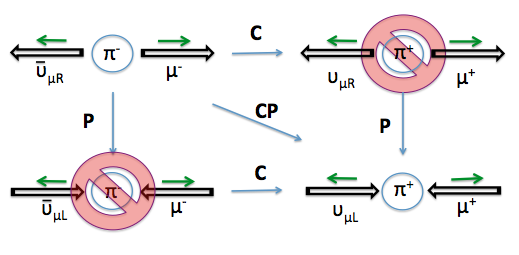
\includegraphics[scale=0.5]{figures/pion_cp}
  \caption[Pion decay]{An illustration of the possible decays of a pion. The black arrow represents the spin vector and the green arrow represents the momentum orientation.}
  \label{fig:cp}
\end{figure}


\subsection{Parity Violation}
\label{sec:pv}
While parity is a conserved quantity in electromagnetic and strong interactions, it is not conserved in the weak interactions. 
In fact, the muon weak decays
\begin{equation}
\begin{split}
&\mu^- \rightarrow {e^-} + \HepAntiParticle{\nu}{e}{} + \nu_{\mu},\\
&\mu^+ \rightarrow {e^+} + \nu_e + \HepAntiParticle{\nu}{\mu}{}
\label{eq:decay}
\end{split}
\end{equation}
are parity violating events, which means that the emitted electrons\footnote{Unless specified, electron refers to both the electron and its antiparticle, the positron.} have a favored direction of emission. 
Because of parity violation in weak processes, a correlation exists between the momentum direction of the decaying electron and the spin orientation of the muon. In other words, there is a preferred direction for the decay of the electron for each spin orientation of the muon. For an illustration of this correlation, the negative muon decay is considered in the two limiting cases of Figure \ref{fig:muon} in the muon rest frame (MRF). Note that the muon momentum and spin are parallel and directed to the right in the laboratory frame to better understand the spin and momentum orientations of the right figure.
 \begin{figure}
  \centering
  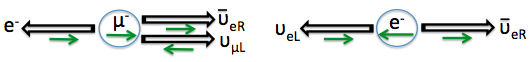
\includegraphics[scale=0.5]{figures/mu_decay}
  \caption[Muon decay]{In the laboratory frame, the muon spin and momentum are parallel and directed to the right. Both decays are in the MRF and show the more likely electron direction. The left decay shows an electron having the maximum possible energy $E_{e,\text{max}}\sim \left(m_{\mu}c^2\right)/2$ = 53 MeV. The right decay shows an electron emitted at rest with its spin antiparallel to its laboratory momentum. }
  \label{fig:muon}
\end{figure}

If the electron has the maximum possible energy in the MRF, the two neutrinos will be emitted back-to-back to the electron with the latter carrying approximately half of the rest mass energy of the muon in order to conserve momentum, $E_{e,\text{max}} \approx \left(m_{\mu}c^2\right)/2$ = 53 Me. \footnote{More precisely, the conservation of energy leads to $\displaystyle E_{e,\text{max}} = \frac{m_{\mu}^2+m_e^2}{2m_{\mu}}c^2$. The above approximation holds when the value $\displaystyle \frac{m_e c^2}{E_{e,\text{max}}} = 9.6\times10^{-3}$ is negligible.}. Parity violation favors the electron to be emitted left-handed which implies that its momentum will be anti-parallel to the muon spin as shown in the left figure. In the case of a zero momentum electron in the MRF, the neutrino and antineutrino will be emitted antiparallel to each other with their spins parallel. Since the electron has a preferred spin direction antiparallel to the muon laboratory momentum, and the muon momentum and spin are parallel. The electron will be emitted parallel to the muon spin as shown on the right figure. These two examples show that by knowing the direction of the decay electron, the muon spin orientation can be inferred. This is the key idea of the muon $g-2$ measurement. By placing muons with the same polarization in a circular orbit within a uniform magnetic field, their longitudinal polarization (their spin component parallel to the momentum vector) will change slightly with each orbit at a rate that is directly related to the anomaly $a_{\ell} = \frac{g_\ell-2}{2}$. The change in the muon longitudinal polarization is determined by using the asymmetric angular distribution of the decay electrons. Formally, the differential decay probability for an electron to be emitted with a normalized energy $y=E/E_{e,max}$ at an angle $\theta$ with respect to the muon spin is given in the MRF with the approximation $E_e \gg m_e c^2$ by
\begin{equation}
dP^{\pm} \propto N\left(E_e\right)\left(1 \pm A(E_e)\cos \theta \right) dy d\Omega,
\label{eq:prob}
\end{equation}
where the $(+)$ is for positive muons decay and the $(-)$ is for negative muons decay and $d\Omega$ is the solid angle. $N\left(E_e\right)$ is a normalization factor that represents the number of decay electrons per unit energy and $A\left(E_e\right)$ is the non-vanishing coefficient of $\cos \theta$ which represents the decay asymmetry factor that reflects the \emph{parity violation}. The expressions of $N\left(E_e\right)$ and $A\left(E_e\right)$ are given by
\begin{equation}
N\left(E_e\right) = 2y^2\left(3-2y\right)  \,\,  \text{and}  \,\,  A\left(E_e\right) = \frac{1-2y}{3-2y}.
\label{eq:na}
\end{equation}
These relations are derived in Appendix \ref{app:muon}.

A few remarks related to Equations (\ref{eq:prob}) and (\ref{eq:na}) are in order. First, the number of decay electrons and asymmetry reach their highest values in the MRF when the energy of the emitted electron is maximum ($y=1$) as shown in Figure \ref{fig:CMF}.
 \begin{figure}
    \centering
  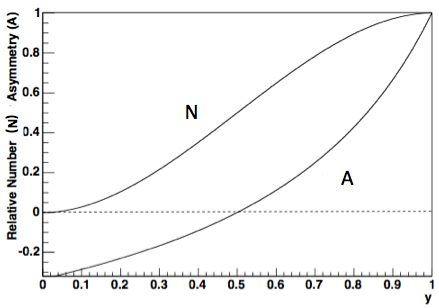
\includegraphics[scale=0.5]{figures/CMF}
   \caption[Decay electrons and asymmetry distributions in the muon rest frame]{The number of decay electrons and the asymmetry distributions in the MRF as a function of the fractional energy $y=E/E_{e,max}$ \cite{bnl}.}
  \label{fig:CMF}
\end{figure}
Also, the asymmetry changes sign at half the maximum energy ($y=\frac{1}{2}$) which means that the emitted electron will have a preferred handedness (or helicity) based on its energy. More importantly, the probability of emitting a specific number of electrons varies with the angle $\theta$ between the electron and the muon spin directions. To be precise, there are more high energy electrons ($e^-$) emitted when their momenta are anti-parallel to the muon ($\mu^-$) spins than when they are parallel. By only selecting the highest energy electrons and counting their number, the spin direction of the muons can be inferred: when the number of electrons is maximum, the muon spin is anti-parallel to the emitted electron direction, and when the number is minimum, the muon spin is parallel to the emitted electron direction. A similar reasoning can be followed for high energy positrons ($e^+$) which will reach a maximum number when the positive muon ($\mu^+$) spins are parallel to the emitted positrons. If the spin of the muons is allowed to precess, then the number of high energy electrons will also precess at the same rate, allowing a direct measurement of the precession frequency. 

\subsection{Relativistic Muons in a Magnetic Field}

In classical electromagnetism, the effect of a uniform magnetic field on a bar magnet is to exert a torque that will align the magnet with the magnetic field. However, if the magnet is spinning, then conservation of angular momentum will cause the bar magnet to precess around the magnetic field. Similarly, the muon has an intrinsic spin and an intrinsic magnetic moment. The interaction of the muon magnetic moment with the magnetic field will cause a precession of the spin around the magnetic field. In fact, it is the expectation value of the spin operator
%\footnote{expectation value vocabulary} 
that precesses around the magnetic field at a constant frequency known as \emph{Larmor frequency}.
This frequency describes the gyration of the spin and is proportional to the magnetic field, thus the name of \emph{gyromagnetic ratio}, $g$. An additional kinematic effect of precession is introduced due to the acceleration of the relativistic reference frame. This is the case for muons moving at high velocities with a transverse acceleration. This precession is derived in Appendix \ref{app:bmt} and is referred to as \emph{Thomas precession}. 

If relativistic muons are constrained to a circular orbit by a uniform magnetic field, as is the case in a \emph{storage ring},\footnote{A storage ring is a circular particle accelerator that maintains particles at the same energy for a long period of time} their spins experience both Larmor and Thomas precessions. The ensemble of these effects on the spin was worked out by Bargmann, Michel and Telegdi in 1959 \cite{bmt}, in an equation known as the BMT equation 
\begin{equation}
\label{eq:bmtS}
\overrightarrow{\omega_s} =  \frac{q}{m_{\mu}c}\left\{\left(a_{\mu} + \frac{1}{\gamma}\right)\overrightarrow{B}    -   a_{\mu}\left(\frac{\gamma}{\gamma + 1}\right)\left(\overrightarrow{\beta} \cdot \overrightarrow{B}\right)\overrightarrow{\beta}   +   \left(a_{\mu}+\frac{1}{\gamma + 1}\right)\overrightarrow{E} \times\overrightarrow{\beta}                 \right\},
\end{equation}
where the velocity is $\displaystyle \overrightarrow{\beta} = \frac{\overrightarrow{v} }{c}$, the Lorentz factor is $\displaystyle \gamma = 1/\sqrt{1-\beta^2}$, $\overrightarrow{E}$ and $\overrightarrow{B} $ are the electric and magnetic fields in the laboratory frame respectively. In addition, the muons also travel in a circular orbit with a frequency known as the \emph{cyclotron frequency} (see Appendix \ref{app:bmt})
\begin{equation}
\overrightarrow{\omega_c} = \frac{q}{\gamma m_{\mu}c}\left\{\overrightarrow{B} + \frac{\gamma^2}{\gamma^2-1} \left(\overrightarrow{E} \times \overrightarrow{\beta}\right)\right\}.
\label{eq:c}
\end{equation}
It is convenient to choose a reference frame which rotates with the velocity vector in order to keep the equations simple. In this case, the precession is given by the difference of angular frequencies $\overrightarrow{\omega_a} = \overrightarrow{\omega_s} - \overrightarrow{\omega_c}$, 
\begin{equation}
\overrightarrow{\omega_a} =   \frac{q}{m_{\mu}c}\left\{a_{\mu}\overrightarrow{B}   -   a_{\mu}\left(\frac{\gamma}{\gamma + 1}\right)\left(\overrightarrow{\beta} \cdot \overrightarrow{B}\right)\overrightarrow{\beta} +   \left(a_{\mu}-\frac{1}{\gamma^2 - 1}\right)\overrightarrow{E} \times\overrightarrow{\beta}                 \right\}.
\label{eq:bmt}
 \end{equation}
If the second and third terms are made to vanish by a proper choice of muon momenta and applied electric and magnetic fields, then Equation (\ref{eq:bmt}) becomes
\begin{equation}
\overrightarrow{\omega_a} =   a_{\mu}\frac{q}{m_{\mu}c}\overrightarrow{B}. 
\label{eq:wa}
\end{equation}
In this case, a nonzero $a_{\mu}$ leads to a precession of the muon spin relative to the cyclotron frequency. This is the central equation of the $g-2$ experiment that will be discussed in the next section. 

\section{Brookhaven $g-2$ Experiment: E821}
\label{sec:exp}
\subsection{Historical Background}
The muon magnetic moment has been measured by three consecutive experiments at CERN through the 1960's and 1970's, and a more recent experiment at Brookhaven National Laboratory (BNL), E821. The last CERN experiment developed a number of novel techniques to measure the anomaly. For instance, it employed a storage ring with a transverse uniform magnetic field to extend the muon's lifetime and cancel the second term in Equation (\ref{eq:bmt}) since in this case $\overrightarrow{\beta} \cdot \overrightarrow{B} = 0$. The experiment chose a specific momentum according to the relation $a_{\mu} -1/\left(\gamma^2-1\right) = 0$ in Equation  (\ref{eq:bmt}) known as the \emph{magic momentum}, which causes the spin oscillation to be independent of any applied electric fields. This equation requires knowledge of the anomaly, which is the quantity the experiment is set to measure. However, the value of the anomaly has already been measured to the first decimal places, which is enough to determine the momentum to the desired precision. The goal of the CERN experiment, on the other hand, was to measure the anomaly to a higher precision. An anomaly value of $a_{\mu} \approx 1.166\times 10^{-3}$ led to a Lorentz factor value of $\gamma_{\text{magic}} \approx 29.30$, and thus the magic momentum is approximately 3.09 GeV in the CERN experiment. 
At the magic momentum, electric quadrupoles\footnote{An electric quadrupole is a system composed of two pairs of oppositely polarized poles placed antiparallel to each other.} were used to provide vertical focusing of the beam. The combined results of the CERN run established a 7.3 ppm precision that was consistent with the standard model prediction. The new measurement techniques developed at CERN were used at Brookhaven with some notable improvements such as the higher intensity of the primary proton beam from the proton storage ring; the direct injection of muons into the storage ring instead of pions; the use of kickers to place muons on the correct orbits; the high field uniformity; and the use of Nuclear Magnetic Resonance probes to map the magnetic field distribution. The E821 experiment resulted in a 14-fold improvement over the CERN experiment where it performed four positive muon runs and one negative muon run which gave a combined precision of 0.54 ppm. In this section, a description of the E821 experiment and the summary of its measurements is given.

\subsection{Description of the Experimental Method}

At BNL, 24 GeV protons are extracted from the proton storage ring Alternating Gradient Synchrotron (AGS) and directed towards a nickel target to generate pions. The pions subsequently decay to muons which pass through selectors that maximize the number of longitudinally polarized muons at the magic momentum of 3.094 GeV/c. These muons are injected into the storage ring via a tangent 1.7 meters long superconducting inflector magnet that provides a 1.5 Tesla vertical field. The field cancels the main storage ring field, allowing the muons to pass almost undeflected into the ring. The muon storage ring has a toroid-shaped structure with a diameter of 14 meters, a beam pipe with a diameter of 90 mm, and a uniform field of 1.45 Tesla. This magnetic field is provided by dipole magnets\footnote{A dipole magnet is a configuration of two opposite pole magnets in the vertical plane of the ring which provide a transverse magnetic field.} that maintain muons in the desired trajectories. However, when the muons are first injected, their trajectories are offset from the storage ring orbit. Pulsed kicker magnets are placed at a specific location in the ring, close to the inflector exit in order to apply a small magnetic field, a ``kick," to adjust the orbit by approximately 10 mrad on each pass. Figure \ref{fig:chain} shows the complete chain of the muon $g-2$ experiment at BNL for positive muons.
 \begin{figure}
    \centering
  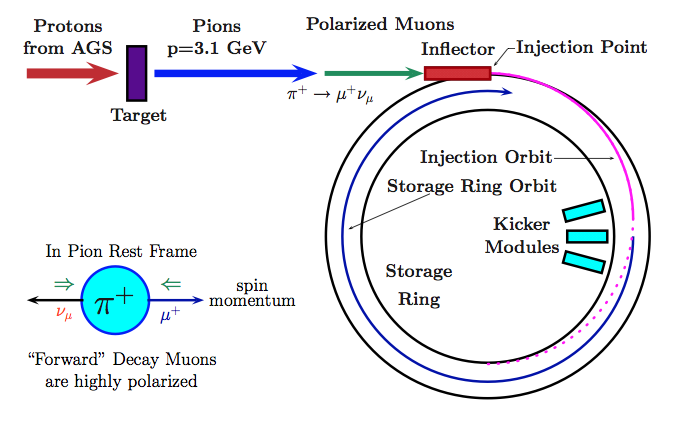
\includegraphics[scale=0.39]{figures/chain}
   \caption[Injection chain in the muon $g-2$ experiment]{The chain of injection and storage of positive muons in the muon $g-2$ ring at BNL. The ``forward'' muons refer to muons decaying in the same direction as the laboratory momenta. In this situation, positive muons have their spins anti-parallel to their momenta \cite{phen}.}
  \label{fig:chain}
\end{figure}

Beam focusing is also needed to constrain the muons within the desired trajectories. Since electric fields do not affect the spin precession, electrostatic quadrupoles are used to continuously focus and defocus the beam in the vertical and the horizontal directions in order to precisely control the beam. 

Muons will travel around the ring at the cyclotron angular frequency described by Equation (\ref{eq:c}), which has a value of approximately 149 ns, and their spin will interact with the magnetic field resulting in a precession with the angular frequency $\omega_s$ given by Equation (\ref{eq:bmt}). However, the electric field $\overrightarrow{E}$ is negligible ($E \approx 0$) and the uniform magnetic field is transverse ($\overrightarrow{\beta} \cdot \overrightarrow{B} = 0$), so the anomalous precession frequency, $\overrightarrow{\omega_a}$, is given by Equation (\ref{eq:wa}) to the first order. Its magnitude is  
\begin{equation}
\omega_a =   a_{\mu}\frac{eB}{m_{\mu}c} 
\label{eq:waa}
\end{equation}

If $g = 2$, then this relative precession $\omega_a$ will be zero, which implies that the muon spin is precessing at the same frequency as the cyclotron frequency. On the other hand, if $g \neq 2$, the muon spin will precess at a different rate than the cyclotron frequency, leading the muon spin axis to change by 12 degrees\footnote{The angular change of spin relative to momentum after one revolution around the ring is $\theta_a = \omega_a T_c$. For $a_{\mu} \approx 1.166\times10^{-3}$, $m_{\mu} = 105.7~\text{Mev/c}^2$, $e = 1.6\times10^{-19}$ C, and $B$ = 1.45 T, $\omega_a \approx 1.45 \times 10^{6}$ Hz and $T_c \approx$ 149 ns, the result using Gaussian units is $\theta_a \approx 12^\circ$.} after each rotation for a constant momentum. Figure \ref{fig:ring} illustrates this change by showing the momentum vector and the projection of the spin vector in the horizontal plane of the storage ring. 
\begin{figure}
  \centering
  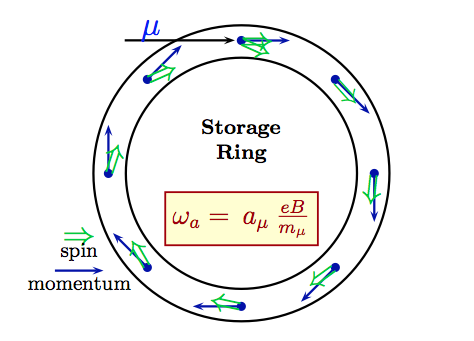
\includegraphics[scale=0.5]{figures/ring}
  \caption[Muon spin precession in the storage ring]{Illustration of the spin precession in the storage ring plane relative to a constant momentum (not to scale). The precession amounts to $\sim$ 12 degrees per orbit \cite{phen}.}
  \label{fig:ring}
\end{figure}
 
In order to determine the anomaly $\displaystyle a_{\mu} = \frac{g_{\mu}-2}{2}$ in Equation (\ref{eq:waa}), three quantities need to be determined accurately: $\omega_a$, $B$, and the muon mass $m_{\mu}$. The muon mass was determined indirectly by an independent experiment on muonium, the bound state of $\mu^+e^-$ \cite{zeeman} as will be discussed. The next two subsections describe the measurement of $\omega_a$ and the magnetic field $B$.

\subsection{Measurement of the Anomalous Angular Frequency $\omega_a$}

As a result of the muons' high momentum ($\sim$ 3.1 GeV), their lifetime is extended from 2.197 $\mu s$ at rest to 64.435 $\mu s$ in the ring. The muons circle the ring many times before they decay into an electron and two neutrinos given by Equation (\ref{eq:decay}). As discussed in Section \ref{sec:pv}, the electron has a preferred emission direction in the muon rest frame that depends on the orientation of the muon spin as given by Equation (\ref{eq:prob}). For example, a positron has a higher probability to be emitted parallel to the muon spin (see Figure \ref{fig:det}). 
\begin{figure}
  \centering
  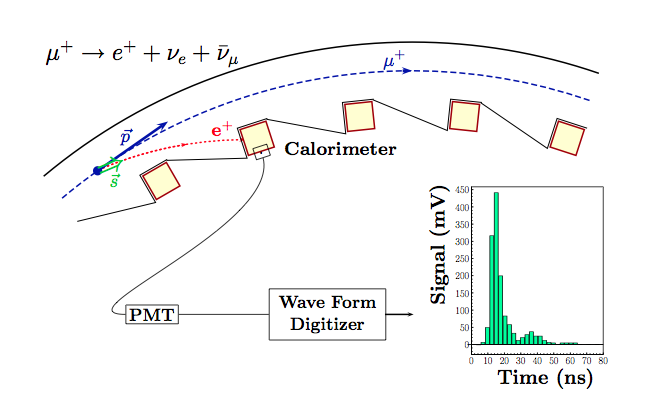
\includegraphics[scale=0.5]{figures/detection}
  \caption[Electron detection in the storage ring.]{A positive muon in the storage ring emits a positron almost parallel to the muon spin (green arrow). The electron is subjected to the same dipole magnetic field which produces a larger deflection leading the positron to interact with the calorimeter scintillator. The light is detected by a Photomultipler Tube (PMT) generating a signal that is digitized by a Wave Form Digitizer \cite{phen}.}
  \label{fig:det}
\end{figure}


If all decay electrons were detected, the number observed will decay exponentially as $\exp(\frac{-t}{\gamma \tau_{\mu}})$. Since the interest is in the precession frequency, a choice of a cut on a laboratory observable that directly depends on this frequency is required. A reasonable choice will permit the selection of a subset of the decay electrons in such a way that their number oscillates at the desired frequency $\omega_a$.  At the magic momentum $p_{\mu} \approx 3.09$ GeV/c, the direction of the electrons cannot be chosen as a cut since most decay electrons are nearly parallel to the muon momentum direction, regardless of their decay orientation in the muon rest frame. Instead, a more practical cut can be applied on the electron's laboratory energy. For instance, if only electrons with the highest possible energy are selected, they will represent positrons that decayed nearly parallel to the muon laboratory momentum with maximum muon rest frame energy. The number of these positrons is larger when they are emitted parallel to the muon spin as opposed to when they are antiparallel. So the number of positrons detected will be maximum when the spin is aligned with the decay positron momentum, and will be minimum when the spin is opposite. It becomes clear that the detected electrons will oscillate with the frequency of the muon spin oscillation $\omega_a$.

In practice, the minimum energy threshold is selected to maximize the \emph{statistical figure-of-merit} (FOM), NA$^2$, in order to minimize the statistical uncertainty. On the left of Figure \ref{fig:LAB}, NA$^2$ is largest for electrons with E$_{th}\approx$ 2.6 GeV ($y \approx .85$). However, the interest is in electrons above an energy threshold. By integrating the quantities N, A, and NA$^2$ for a single electron threshold as a function of the energy threshold, NA$^2$ is maximized at E$_{th}\approx$ 1.8 GeV as shown on the right of Figure \ref{fig:LAB}. 
\begin{figure}
\begin{subfigure}
  \centering
  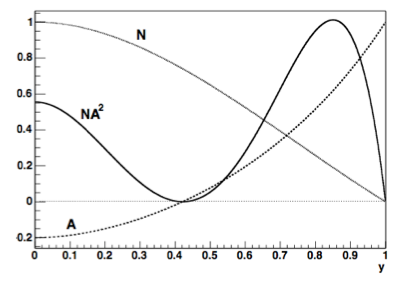
\includegraphics[scale=0.5]{figures/NA_time}
%\caption{(a)}% N, A, NA$^2$}
%   \caption[Decay electrons and asymmetry distributions in the laboratory frame.]{The equivalent of Figure \ref{fig:CMF} boosted to the laboratory frame. The fractional energy is $y=E/E_{e,max}$ where $E_{e,max} \approx 3.098$ GeV. The quantity $NA^2$ represents the \emph{statistical figure-of-merit}. It needs to be maximized in order to achieve a minimum statistical uncertainty. \cite{bnl}}
  %\label{fig:LAB}
  \end{subfigure}
\begin{subfigure}
  \centering
  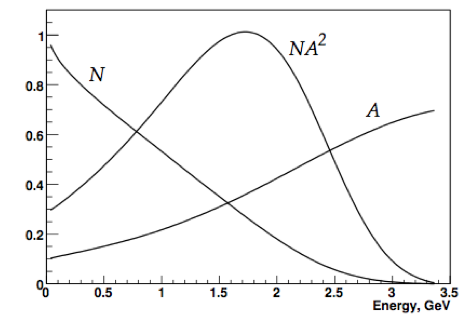
\includegraphics[scale=0.44]{figures/NA_integrated}
%\caption{(b)}% Integrated N, A, NA$^2$}
%   \caption[Decay electrons and asymmetry distributions in the laboratory frame.]{The equivalent of Figure \ref{fig:CMF} boosted to the laboratory frame. The fractional energy is $y=E/E_{e,max}$ where $E_{e,max} \approx 3.098$ GeV. The quantity $NA^2$ represents the \emph{statistical figure-of-merit}. It needs to be maximized in order to achieve a minimum statistical uncertainty. \cite{bnl}}
  %\label{fig:LAB2}
  \end{subfigure}
\caption[Decay electrons and asymmetry distributions in the laboratory frame.]{The equivalent of Figure \ref{fig:CMF} boosted to the laboratory frame. Left: N, A, and NA$^2$ as a function of the fractional energy $y=E/E_{e,max}$ where $E_{e,max} \approx 3.098$ GeV. Right: Integrated N, A, and NA$^2$ as a function of the threshold energy \cite{bnl}.}
\label{fig:LAB}
\end{figure}

With the the assumption that the spin precession vector is independent of time, the angle between the spin component in the orbit plane and the muon momentum is $\omega_at+\phi$, where $\phi$ is a constant phase. At time t, the number of decay positrons N(t) with energy larger than the threshold energy E$_{th}$ is
\begin{equation}
N(t, E_{th}) = N_0(E_{th})\exp \left(\frac{-t}{\gamma \tau_{\mu}}\right) \left[1 + A(E_{th})  \sin\left(\omega_a t + \phi(E_{th})\right)\right],
\label{eq:fit}
\end{equation}
where N$_0$ is a normalization factor and A is the asymmetry factor for positrons of energy greater than E$_{th}$. 
\begin{figure}
  \centering
  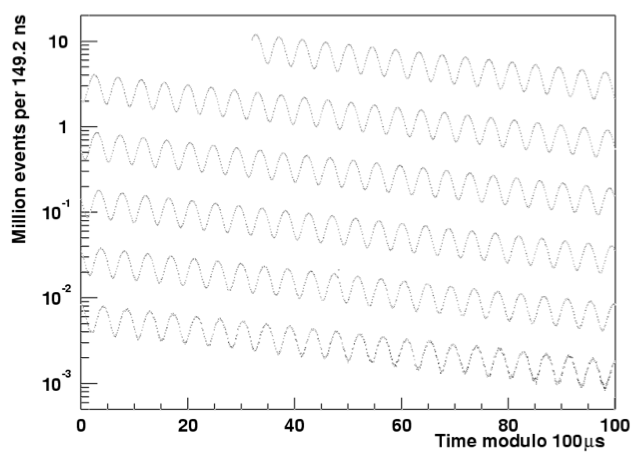
\includegraphics[scale=0.5]{figures/oscillation}
  \caption[Histogram of detected electrons]{Histogram of the 3.6 billion detected electrons above 1.8 GeV as a function of time, modulo 100 $\mu s$, for the 2001 data set \cite{bnl}.}
  \label{fig:osc}
\end{figure}
Figure \ref{fig:osc} shows the arrival-time spectrum of the final E821 data run for 2001. As discussed earlier, the spectrum follows an exponential decay of the muons modulated by the $g-2$ dependent angular frequency. By fitting this time distribution to the five-parameter function of Equation (\ref{eq:fit}), the angular frequency $\omega_a$ is determined.

The electron detection is made via 24 symmetrically distributed calorimeters inside of the ring as shown in Figure \ref{fig:det}. The goal of the calorimeters is to determine the electrons' energy and arrival time. The calorimeters are designed to detect the high energy electrons where 65\% of the electrons with energy higher than 1.8 GeV are intercepted \cite{bnl}. Each calorimeter is made out of plastic-scintillator\footnote{A plastic-scintillator causes the particle to deposit energy when it passes through. The scintillator re-emits the absorbed energy in the form of light. } material (52\% lead alloy, 38\% scintillating fiber, and 10\% epoxy) read out by photomultiplier tubes\footnote{Photomultiplier tubes are light detectors that operate via the photoelectric effect where photons, upon hitting a photocathode, generates a cascade of electrons that can be read by a Wave Form Digitizer.} (PMTs). The decaying electrons have both tangential and radial momentum components. However, the radial component is quite small, which permits the extrapolation of the electron's trajectory from the calorimeter to the central muon orbit, allowing a measurement of the decay position and vertical angle as shown in Figure \ref{fig:det}. The muon position information is particularly important in characterizing the magnetic field felt by the muon at that specific location. 
% BNL p34 
Finally, a Wave Form Digitizer (WFD) captures raw analog PMT signals and digitizes them for further processing with the advantage of maintaining high resolution measurements. An example of a WFD output is shown in Figure \ref{fig:det}.

\subsection{Measurement of the Magnetic Field $B$}

The magnetic field $B$ is weighted by the stored muons distribution and averaged over the running time. It can be expressed as an integral of the product of the muon distribution multiplied by the magnetic field distribution over the storage region leading to a coupling of the moments of the muon distribution to the respective multipoles of the magnetic field. In order to determine the weighted magnetic field $B$ to sub-ppm precision, either the moments and multipoles of the muon and magnetic field distributions should be known extremely well, or a particularly uniform magnetic field and a circular beam aperture should be used so that the leading term dominate the multipole expansion of the magnetic field. The latter option was selected where \emph{Nuclear Magnetic Resonance} (NMR) permitted the determination of the magnetic field to the tens of ppb. In this experiment, NMR is based on using protons in a water sample placed in the dipole magnetic field, and exposed to a $\frac{\pi}{2}$ radio-frequency (RF) pulse which rotates the net magnetization of the protons.\footnote{A radio-frequency pulse is a pulse in the range from 3 KHz to 300 GHz that excites a large frequency band resulting in the appearance of a time-dependent magnetic field which can rotate the magnetization vector of the protons.} A pickup coil placed in the transverse direction registers the induced signal that exponentially decays with an oscillation as the protons' magnetization vector regains its equilibrium position. This process is known as \emph{Free Induction Decay}, which has a frequency sensitive to the the local magnetic field value. 

The NMR procedure allows the determination of the magnetic field at thousands of points around the ring which permits the mapping and monitoring of the field during data taking. A calibration method is used to express the Larmor spin frequency of a proton in a water sample in terms of the Larmor spin frequency of a free proton $\omega_p$. The Larmor frequency of a free proton is $\omega_p=\gamma_pB$, where $\gamma_p$ is the free proton gyromagnetic moment ratio given by Equation (\ref{eq:mu}) such that $\overrightarrow{\mu_p} = \gamma_p \overrightarrow{S}$. Hence, the free proton frequency, $\omega_p$, is related to the magnetic moment of the free proton $\mu_p$ and the magnetic field $B$ by 
\begin{equation}
B = \frac{\hbar\omega_p}{2\mu_p}.
\label{eq:wp}
\end{equation} 
According to the last equation, this weighted magnetic field can be referred to as $\omega_p$. 
By writing Equation (\ref{eq:mu}) in the form $\displaystyle \frac{q}{mc} = \frac{2\mu_{\mu}}{1+a_{\mu}}$ and using Equations (\ref{eq:waa}) and (\ref{eq:wp}), the anomaly can be written in terms of dimensionless ratios,
\begin{equation}
a_{\mu} = \frac{\mathcal{R}}{\lambda - \mathcal{R}},
\label{eq:R}
\end{equation}
where $\displaystyle \lambda \equiv \frac{\mu_{\mu}}{\mu_{p}}$ and $\displaystyle \mathcal{R} \equiv \frac{\omega_a}{\omega_p}$.
The muon-to-proton magnetic moment ratio, $\lambda$, embodies in it both the muon and the proton masses since $\displaystyle \frac{\mu_{\mu}}{\mu_{p}} = \frac{g_{\mu}}{g_p}\frac{m_p}{m_{\mu}}$. Its value is determined through a precision measurement of the Zeeman ground state hyperfine transitions in muonium ($\mu^+e^-$) by E1054 LAMPF at Los Alamos \cite{zeeman},
\[\lambda_+ = \frac{\mu_{\mu^+}}{\mu_{p}} = 3.183\, 345\, 137\, (85).\] 
Note that this result has a precision of $\sim 27$ ppb which could not be obtained by mass measurements. The use of $\lambda_+$ to determine $a_{\mu^-}$ implies CPT invariance.\footnote{CPT invariance implies that the product of the three discrete transformations C, P, and T taken in any order is a symmetry of theories like the SM. It guarantees that particles and antiparticles have the same masses and lifetimes.} In other words, the relations $a_{\mu^-} = a_{\mu^+}$ and $\lambda_+ = \lambda_-$ must be valid. In fact, the measurement of $\omega_a$ for positive and negative muons provides a CPT test where 
\begin{equation}
\Delta \mathcal{R} = \mathcal{R}_{\mu^-} - \mathcal{R}_{\mu^+} = \left(3.6 \pm 3.7 \right) \times 10^{-9}.
\end{equation}

\subsection{Corrections and Systematic Errors}

The method described so far presents an ideal scenario. However, there are additional effects that affect the measurements, the most important of which are related to the beam dynamics leading to a displacement of the beam trajectory and the determination f the magnetic field at a location offset from the orbit of the muons.  
While the dipole magnetic field insures the bending of the muon beam, the vertical focusing is done via electric quadrupoles. These quadrupoles set an electric field gradient that causes the beam to oscillate around its equilibrium in the plane transverse to the beam. This type of oscillation is known as the \emph{betatron oscillation} and it satisfies the harmonic oscillator equations 
\begin{equation}
\begin{split}
\ddot{x} + \omega_x^2 x = 0, \\
\ddot{y} + \omega_y^2 y = 0,
\end{split}
\end{equation}
where the frequencies are defined as
\begin{equation}
\begin{split}
\omega_x = \omega_c\sqrt{1-n}, \,\,\,\,\,\,\,\,
\omega_y = \omega_c\sqrt{n},
\end{split}
\end{equation}
where $ \omega_c$ is the cyclotron frequency and n is the field index defined as 
\begin{equation}
n = \frac{R_0}{\beta B_0}\frac{\partial E_y}{\partial y},
\end{equation}
with an orbit stability condition of $0<n<1$ and where $R_0$ is the equilibrium radius, $B_0$ is the dipole magnetic field, and $\beta$ is the muon speed. Since the betatron frequencies are smaller than the cyclotron frequency, this type of focusing is called \emph{weak focusing}.
 
The betatron motion perturbs the muons trajectories affecting the muons momenta and directions. This implies that the assumptions $\overrightarrow{\beta} \cdot \overrightarrow{B} = 0$ and $a_{\mu} -1/\left(\gamma^2-1\right) = 0$ ($E \approx 0$) are no longer valid. These effects should be taken into account in determining the anomalous frequency $\omega_a$ as given by Equation (\ref{eq:wa}). The correction for the momentum direction to satisfy $\overrightarrow{\beta} \cdot \overrightarrow{B} = 0$ is called the \emph{Pitch Correction}. Similarly, the momentum spread from the magic momentum requires a correction to the electric field referred to as the \emph{Radial Electric Field Correction}. The combination of these two corrections are explicitly shown in column 4 of Table \ref{tab:R} (E/pitch). 

Next, the sources of systematic errors in $\omega_a$ are briefly defined with their numerical values listed in Table \ref{tab:sys}:
\begin{itemize}
\item Pileup: Two low-energy electrons that reach the detector at very close times can be interpreted as one high-energy electron.        
\item AGS background: Mis-steering the proton beam in the AGS might lead it to hit a part of the target that produces a higher flux of pions entering the storage ring when muons are injected. %p11
\item Lost muons: Small perturbations in the magnetic or electric fields may couple to betatron oscillations at their resonant frequency leading to a motion without bound until the muons are lost.
\item Timing shifts and gain changes: A calibration pulse was sent in parallel to the beam data through the optical and electronic readout system to monitor the time resolution of the detector and variations in the energy scale used.
\item Fitting/Binning: The electron decay spectra was sorted into discrete energy bins and fitted to a multi-parameter fitting function for different data subsets which introduced errors related to the corrections applied to the spectra and the experimental conditions. 
\item Coherent Betatron Oscillation (CBO): Mismatch between the inflector and storage ring apertures at the injection point causes the beam to alternatively widen and narrow as it circulates around the ring. 
\end{itemize}
\begin{table}
  \caption[Systematic errors for $\omega_a$]{Systematic errors for $\omega_a$ for the three high-statistics running periods. ${\dagger}$ In the 2001 run, the AGS background, timing shifts, E field and pitch correction, binning and fitting procedure have a total systematic error of 0.11ppm. }
  \label{tab:sys}
  \centering
  \begin{tabular}{*{4}{l}}
	\hline \hline
      Years   & 1999 & 2000  & 2001 \\ 
      %$\sigma_{sys}$($\omega_a$)
       & (ppm) & (ppm) & (ppm)\\
      \hline
       Pileup & 0.13 & 0.13 & 0.08  \\
       AGS background & 0.10 & 0.01 &    ${\dagger}$\\
       Lost Muons & 0.10 & 0.10 & 0.09  \\
       Timing Shifts & 0.10 & 0.02 &    ${\dagger}$\\
       E-field and pitch & 0.08 & 0.03 &    ${\dagger}$\\
       Fitting/Binning & 0.07 & 0.06 &    ${\dagger}$\\
       CBO  & 0.05 & 0.21 & 0.07  \\
       Gain Changes & 0.02 & 0.13 & 0.12   \\ \hline
       Total systematic error on $\omega_a$ & 0.3 & 0.31 & 0.21  \\
         \hline  \hline
     \end{tabular}
\end{table}

The systematic uncertainties in the magnetic field measurement are due to effects related to the determination of the precession frequency of protons in a water sample placed in a trolley probe that is offset from the orbit of the muons. The positioning of the trolley permits measurements of the magnetic field during data taking at multiple locations around the ring. However, the magnetic field at the trolley's position might vary from the field that muons experience. In addition, the desired quantity is the free proton precession, but the measured quantity is the proton's precession in water. For these reasons, uncertainties are introduced in the processes of calibration and interpolation. Table \ref{tab:wp} summarizes the numerical values of the errors in $\omega_p$ for three running periods.
\begin{table}
  \caption[Systematic errors for $\omega_p$]{Systematic errors for $\omega_p$ for the three high-statistics running periods. $\dagger$ After 1999, the inflector, which was damaged, was replaced making the disturbance of the inflector's fringe field on the main storage ring field negligible.}
  \label{tab:wp}
  \centering
  \begin{tabular}{*{4}{l}}
	\hline \hline
      Years   & 1999 & 2000  & 2001 \\ 
      %$\sigma_{sys}$($\omega_a$)
       & (ppm) & (ppm) & (ppm)\\
      \hline
       Absolute calibration of standard probe & 0.05 & 0.05 & 0.05  \\
       Calibration of the trolley probes & 0.20 & 0.15 & 0.09 \\
       Trolley measurements of $B$ & 0.10 & 0.10 & 0.05  \\
       Interpolation with fixed probes & 0.15 & 0.10 &  0.07 \\
       Uncertainty from muon distribution & 0.12 & 0.03 & 0.03 \\
       Inflector fringe field uncertainty & 0.20 & $\dagger$ &  $\dagger$  \\
       Others  & 0.15 & 0.10 & 0.10     \\ \hline
       Total systematic error on $\omega_p$ & 0.4 & 0.24 & 0.17 \\ \hline  \hline
     \end{tabular}
\end{table}

The electric dipole moment (EDM) of the muons should also be mentioned for completeness of the discussion. Just as the magnetic moment originates from the current of the spinning charged lepton and interacts with the magnetic field, the EDM is due to the electric charge of the lepton and it interacts with the electric field. The equivalent of Equation (\ref{eq:mu}) for the EDM is  
\begin{equation}
\overrightarrow{d} = \eta\frac{q}{2mc}\overrightarrow{S}
\label{eq:d}
\end{equation}
where $d$ is the dimensionless constant equivalent to the g-factor. Equation (\ref{eq:R}) assumes a zero muon EDM. For a non-zero muon EDM, the spin frequency is 
\begin{equation}
\overrightarrow{\omega} = \overrightarrow{\omega}_a + \overrightarrow{\omega}_{EDM} = \overrightarrow{\omega}_a
-\frac{q\eta}{2mc}\left( \overrightarrow{\beta}\times \overrightarrow{B} \right)
\label{eq:edm}
\end{equation}
However, the current experimental value for muons is $d_\mu = \left(-0.1 \pm 0.9\right) \times 10^{-19} e \cdot \text{cm}$ \cite{pdg}, which is too small to affect the anomalous precession frequency $\omega_a$.

\subsection{Summary of Results from E821}

The experiment E821 has conducted four positive muon runs (1997-2000) and one negative muon run (2001) that are all reported in \cite{bnl}. The results of the experiment for the last three runs with the largest statistics are displayed in Table \ref{tab:R} and Table \ref{tab:amu}.
\begin{table}
  \caption[Results for the anomalous precession frequency $\omega_a$]{Results for the anomalous precession frequency $\omega_a$ including the relative electric field and pitch corrections shown in column 4 and the event-weighted magnetic field $\omega_p$ given with their uncertainties. The error on the average takes into account the correlated systematic uncertainties between different periods.}
  \label{tab:R}
  \centering
  \begin{tabular}{*{6}{c}}
	\hline \hline
      Years  & Electrons & $\omega_a/(2\pi)$& E/pitch & $\omega_p/(2\pi)$ & $\mathcal{R} = \omega_a/\omega_p$\\ 
      &[millions] &  [Hz]  &  [ppm]  & & \\
      \hline
       1999 ($\mu^+$) & 950 & 229\,072.8(3) & 0.81(8) & 61\,791\,256(25)& 0.003\,707\,204\,1(51)  \\
       2000 ($\mu^+$) & 4000 & 229\,074.11(16) & 0.76(3) & 61\,791\,595(15)& 0.003\,707\,205\,0(25)  \\
       2001 ($\mu^-$)  & 3600 & 229\,073.59(16) & 0.77(6) & 61\,791\,400(11)& 0.003\,707\,208\,3(26)  \\  \hline
       Average & & & & & 0.003\,707\,206\,3(20) \\
         \hline  \hline
     \end{tabular}
\end{table}
\begin{table}
  \caption[BNL E821 results of the anomaly $a_{\mu}$]{BNL E821 results of the anomaly $a_{\mu}$ for the three high-statistics running periods. }
  \label{tab:amu}
  \centering
  \begin{tabular}{*{4}{c}}
	\hline \hline
      Years  & Polarity & $a_{\mu}\times 10^{10}$ & Precision [ppm] \\ \hline
       1999 & $\mu^+$ & 11\,659\,202(15) & 1.3  \\
       2000 & $\mu^+$ & 11\,659\,204(9) & 0.73  \\
       2001 & $\mu^-$ & 11\,659\,214(9) & 0.72  \\ \hline
       Average & & 11\,659\,208.0(6.3) & 0.54\\
         \hline  \hline
     \end{tabular}
\end{table}

The averaged value of the ratio $\mathcal{R} = \omega_a/\omega_p$ of Equation (\ref{eq:R}) evaluated in the cases of negative and positive muons is
\begin{equation}
\mathcal{R}_{\mu}\left(\text{E821}\right) = 0.003\,707\,206\,4(20).
\end{equation}
The anomalous magnetic moment is thus 
\begin{equation}
a_{\mu}^{\text{E821}} = 11\, 659\, 208  \left(5.4\right)_{stat}  \left(3.3\right)_{sys}  \left(6.3\right)_{tot} \times 10^{-10} \,\,\,\,\,\,\, \left(0.54  \text{ ppm}\right)
\end{equation}
This final measurement has a statistical uncertainty of 0.46 ppm and a systematic uncertainty of 0.28 ppm which were added in quadrature to get a total uncertainty of 0.54 ppm. In order to improve the statistical uncertainty to the same level as the systematic uncertainty, an additional running period of 8 years is required. Alternatively, the experiment can use a higher intensity beam to produce more electrons, and thus more statistics. This is precisely what the new Fermilab experiment does.

\section{Future Fermilab $g-2$ Experiment: E989}

The Fermilab experiment, E989, will measure the anomaly $a_{\mu}$ with an error of $1.6 \times 10^{-10}$ leading to a fractional error of 0.14 ppm, where the level of the statistical and systematic uncertainties are both at the 0.10 ppm level. In order to achieve this goal, a collection of data that is twenty-one times larger than the E821 data collection is required, which scales to $1.8\times10^{11}$ detected positrons with energy greater than 1.8 GeV and arrival time greater than 30 $\mu s$ after muon injection in the storage ring. Since the detected positron number is directly proportional to the protons on target, the Fermilab experiment will have to deliver $4\times10^{20}$ protons. Indeed, it will be possible to reach these numbers by using the Fermilab beam complex which is expected to annually deliver $2.3 \times 10^{20}$ 8 GeV protons on an Inconel\footnote{Inconel is an alloy, composed of a metal and other elements, specifically designed to withstand high beam stresses.} core target. At this rate, the desired number of protons, and thus positrons, will be achieved in less than two years of running. 

Fermilab will improve upon the methods and instrumentation used at BNL. For instance, the produced pion beam will pass through a bending magnet to select particles with a momentum of 3.1 GeV ($\pm$ 10 \%), and subsequently traverse a decay line of over one kilometer, which results in a pure muon beam entering the storage ring. The muon storage ring will be filled at a repetition rate of 15 Hz compared to 4.4 Hz at BNL, and the stored muon-per-proton ratio will also be increased by a factor of 5 to 10 times. The muons will enter the ring via a new superconducting inflector, characterized by a limited flux leakage onto the storage region and a larger horizontal beam aperture to allow a higher storage efficiency. The muon kicker will have an optimized pulse-forming network\footnote{A pulse-forming network is an electric circuit composed of capacitors that provide a square pulse with a flat top upon discharge.} that will provide a pulse close to the beam width, as opposed to the E821 kicker which had a pulse width longer than the cyclotron period. At BNL, the injected muon beam was contaminated with pions which introduced a hadronic flash background. This background will be reduced by a factor of 20 in E989.\\
E989 will use the same muon storage ring of E821, which has been relocated to Fermilab in the summer of 2013 in a new building characterized by mechanical stability and controlled temperature. These options were not available at BNL.

The new segmented calorimeters will use silicon Photomultipliers (SiPMs) to read signals from lead-fluoride crystal (PbF$_2$). The crystal has an improved energy resolution and a very fast Cherenkov signal\footnote{A Cherenkov signal is due to Cherenkov radiation which is an electromagnetic radiation produced when a particle travel through a dielectric material with a velocity greater than the phase velocity of light in that dielectric. While no particle travels faster than light in vacuum, the situation is different in a dielectric since $v_\text{light}$ = c/n with n $>$1.} response. When a photon strike a SiPM pixel, it generates an avalanche that is linearly combined with the other pixels that were hit to form the response. SiPMs are designed so that their number of pixels exceed the number of photons that are expected to strike the device allowing a high photo-detection efficiency. The added benefit of using SiPMs is that they can be placed inside the storage ring at the back of the PbF$_2$ crystals without perturbing the field, as opposed to PMTs which require long lightguides. 

Since momentum spread, betatron oscillations, and muons distribution introduced ppm level corrections in the anomalous precession at BNL, E989 introduces in-vacuum straw drift tubes\footnote{A straw tube for high resolution position measurement is constructed with an anode wire centered within a cathode tube and maintained at a potential difference in a gas environment.  When a charged particle passes through the tube, it ionizes the gas generating a signal for a particle ``hit'.' } as tracking detectors to better understand beam dynamics, limit pile up effects, and provide an independent validation of the systematic uncertainties analysis (for example, an independent momentum measurement.) In addition, it will also be used to search for a permanent EDM. The electronics and data acquisition systems will be upgraded to handle the increased rate of data taking and to record all information related to the run for monitoring and the application of corrections in the analysis stage. 

Last but not least, the storage ring magnetic field, and thus $\omega_p$, will be measured with an uncertainty that is approximately 2.5 times smaller by placing critical NMR probes at strategic locations around the ring and shimming the magnetic field to achieve a high uniformity in addition to other incremental adjustments. \cite{e989}


\section{The Standard Model Evaluation of the Anomaly $\left(a_{\mu}\right)$}
\label{sec:sm}
\subsection{Introduction}
The magnetic moment of the muon is described by Equation (\ref{eq:mu})
\begin{equation}
\begin{split}
\overrightarrow{\mu} = g\frac{q}{2mc}\overrightarrow{S}, \,\,\,\,\,\,\,\,\,\,  g = 2\left(1+a_{\mu}\right),
\label{eq:mug}
\end{split}
\end{equation}
where $g=2$ in the Dirac theory. Particles with $g=2$ are referred to as Dirac particles. The anomaly $a_{\mu}$ is due to quantum fluctuations that couple the muon spin to virtual fields which leads to contributions that can be calculated in the SM theory. For instance, the three interactions that the SM describes are electromagnetic interactions by Quantum Electrodynamics (QED), hadronic strong interactions by Quantum Chromodynamics (QCD), and weak interactions by the Electro-Weak theory (EWT). In this language, the anomaly can be written as the sum of contributions from each theory as
\begin{equation}
a_{\mu}^{SM} = a_{\mu}^{\text{QED}}+a_{\mu}^{\text{Hadronic}}+a_{\mu}^{\text{EW}}.
\label{eq:asm}
\end{equation}

The QED and weak contributions to the anomaly are well understood and have been evaluated using perturbation theory to a high precision leading to small errors, and thus permitting the comparison with experimental results. On the other hand, the hadronic contribution limits the accuracy of the theoretical prediction since these effects cannot be evaluated using perturbation methods at low energies. For this reason, the hadronic contribution has to be evaluated using experimental data via a dispersion relation, and thus leading to the highest uncertainty in the prediction.

\subsection{The QED Contribution to $a_{\mu}$}

The mediator of electromagnetic processes involve the interactions between charged particles is the photon. In a loose language, sometimes the muon will ``recapture'' the photon it emitted and thus forming a new ``Dirac muon + photon'' system.
If the magnetic moment of the muon is probed at that instant, it will be different from 2 since the configuration does not have just a Dirac muon. Similarly, there can be more than one photon or even electron-positron pairs that form a new system, and thus the contributions to $g$ of Equation (\ref{eq:mug}) can be expressed as a series in the form: Dirac muon + \{Dirac muon + photon\} + \{Dirac muon + several photons\} + \{electron + positron\} \ldots.

Formally, the dominant contribution is that of the lowest-order (LO) QED process that involves the exchange of a virtual photon and is represented by a one-loop diagram as illustrated in Figure \ref{fig:schwinger}. This contribution is known as the \emph{Schwinger term} and it is common to all three charged leptons. Its value is calculated in Appendix \ref{app:schwinger} and the result is 
\begin{equation}
a_{\mu}^{\text{QED,LO}} = \frac{\alpha}{2\pi} \approx 1.16 \times 10^{-3},
\label{eq:schwinger}
\end{equation}
where $\alpha$ is the fine structure constant that has been measured experimentally in the $^{87}$Rb atom with 0.66 ppb precision and has an inverse value of 
\begin{equation}
\alpha^{-1} \left(\text{Rb}\right)= 137.035\,999\,049(90) \,\,\cite{alpha}.
\end{equation}
Equation (\ref{eq:mug}) can be written to first order in $\alpha$ representing the first-order term in the one-loop diagram contribution that will be calculated in Appendix \ref{app:schwinger}
\begin{equation}
g = 2\left(1+\frac{1}{2}\frac{\alpha}{\pi}+ \mathcal{O}\left(\left(\frac{\alpha}{\pi}\right)^2\right)\right),
\label{eq:schwinger2}
\end{equation}
where the higher-order corrections to QED processes are suppressed by increasing powers of $\alpha$.  
\begin{figure}
  \centering
  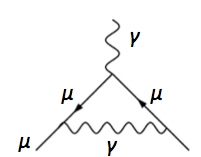
\includegraphics[scale=0.5]{figures/schwinger}
   \caption[Feynman diagram of the lowest-order contribution]{The lowest-order (Schwinger) contribution to the muon magnetic moment anomaly \cite{thesis}.}
\label{fig:schwinger}
\end{figure}
In fact, the QED calculation has been carried out to the fifth-loop contribution 
\begin{equation}
a_{\mu}^{\text{QED}} = 116\,584\,71.895 \,\, (0.009)(0.019)(0.007)(0.077) \times 10^{-10} \,\,\cite{qed}
\label{eq:qed}
\end{equation} 
with the uncertainties corresponding to the lepton mass ratios, the fourth-order term in the four-loop contribution, the fifth-order term in the five-loop contribution, and the value of the fine structure constant $\alpha \left(\text{Rb}\right)$. It should be noted that this contribution accounts for over 99.99\% of the total contribution to the muon magnetic moment anomaly with much smaller uncertainties than the experimental value.

\subsection{The Weak Contribution to $a_{\mu}$}

The weak contribution is the smallest correction to the anomaly. The current electroweak calculation is performed up to two loops.
The leading electroweak effect originates from the single loop diagrams of Z and W$^{\pm}$ bosons shown in Figure \ref{fig:weak} with a result of 
\begin{equation}
a_{\mu}^{\text{EW(1)}} = 19.48 \times 10^{-10} \,\,\cite{ew1}.
\end{equation}
\begin{figure}
  \centering
  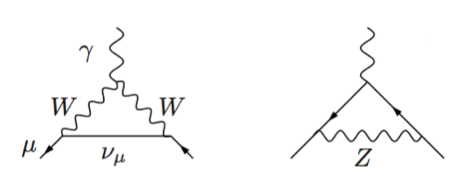
\includegraphics[scale=0.5]{figures/wz}
   \caption[Feynman diagram of a weak contribution]{Weak contributions to the muon anomalous magnetic moment with a one-loop diagrams with virtual W and Z gauge bosons \cite{thesis}. }
  \label{fig:weak}
\end{figure}
The two-loop contribution is negative which reduces the weak contribution, and the third-loop contribution is negligible leading to a total result of 
\begin{equation}
a_{\mu}^{\text{EW}} = 15.36(1.0) \times 10^{-10} \,\,\cite{ew},
\label{eq:ew}
\end{equation}
where the error is due to unknown higher order contributions. Nevertheless, the error is very small.
Since the weak contribution to the anomaly is of the order of 1.3 ppm, the 0.54 ppm precision of E821 allowed this experiment to be the first to probe the weak scale of the SM at this precision and subsequently test $a_{\mu}^{\text{EW}}$. Moreover, the value of the EW contribution is smaller than the current discrepancy between experiment and theory as given in Equation (\ref{eq:diff}).

\subsection{The Hadronic Contribution to $a_{\mu}$}

The hadronic contribution is the second largest contribution, which constitutes about 60 ppm of the total value of $a_{\mu}$ with a dominant error of about 0.4 ppm. 
This contribution is divided into three pieces: the lowest-order (LO) and higher-order (HO) vacuum polarization (VP) contributions, and the light-by-light (LbL) scattering contribution. Hence, $a_{\mu}^{\text{Had}}$ can be expressed as
\begin{equation}
a_{\mu}^{\text{Had}} = a_{\mu}^{\text{Had,LOVP}}+a_{\mu}^{\text{Had,HOVP}} + a_{\mu}^{\text{LbL}}.
\end{equation}
Schematics of these three contributions are shown in Figure \ref{fig:had}.
\begin{figure}
  \centering
  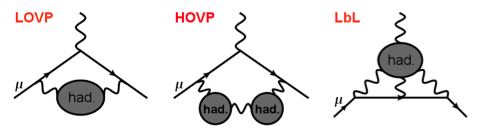
\includegraphics[scale=0.5]{figures/had}
   \caption[Feynman diagram of some hadronic contributions]{The Feynman diagrams for the three different hadronic contributions to $a_{\mu}$ \cite{thesis}.}
  \label{fig:had}
\end{figure}

VP refers to the partial screening of the charge of a particle by the vacuum which plays the role of a dielectric medium. In the case of the hadronic contribution to the muon anomaly, the virtual photon of Figure \ref{fig:schwinger} may lead to the virtual creation and re-absorption of quark pairs and the corresponding hadrons, schematically represented in Figure \ref{fig:had} by ``had.'' corresponding to all possible hadronic states. The electromagnetic and weak interactions have small coupling constants which makes the higher terms in the perturbative expansion of the anomaly negligible. But the strong interactions have a small coupling only at high energies, which prevents the use of perturbative methods at low energies. Generally, the energy region below 2 GeV cannot be treated using perturbative QCD. The virtual hadrons that affect the anomaly have an energy scale of $m_{\mu}c^2 \approx 106$ MeV which is well below the perturbative QCD region. For this reason, a semi-phenomenological method that uses experimental input from hadronic $e^+e^-$ annihilation data to evaluate the LO and HO VP contributions is employed. This method, which make use of a dispersion relation, connects the photon VP due to hadronic contributions shown in the two left diagrams in Figure \ref{fig:had} to the total $e^+e^- \to \text{hadrons}$ cross section at low energies which is obtained from experimental data. The improvement in the measurement of $e^+e^-$ annihilation to hadrons at low energies have been the focus of several experiments. Some of the experiments are CMD2 and SND collaborations in Novosibirsk (Russia); the KLOE collaboration at Frascati (Italy); and the BaBar at SLAC (USA). It should be noted that there is an alternative method in evaluating the VP contributions by using the $\tau$-decays. 
One of the most recently reported LO hadronic contribution is 
\begin{equation}
a_{\mu}^{\text{Had,LOVP}} = 6\,94.9(4.3) \times 10^{-10} \,\,\cite{hadlo2}. 
\label{eq:hadlo2}
\end{equation}
While the HO hadronic contribution is given by 
\begin{equation}
a_{\mu}^{\text{Had,HOVP}} = -9.84(0.07) \times 10^{-10} \,\,\cite{hadlo2}. 
\label{eq:hadho}
\end{equation}

The hadronic LbL contribution, shown in the far right schematic of Figure \ref{fig:had}, is of the order of $\mathcal{O}\left(\alpha_s^3\right)$ which is quite small. Since the process involves three virtual photons, the use of experimental data to evaluate the LbL contribution is not possible. Instead, the contribution is evaluated based on hadronic models with the requirement that they correctly reproduce the QCD properties. The downside of this approach is that the final result is model dependent. Currently, active research work is being done in this area. One of the calculations obtained is 
\begin{equation}
a_{\mu}^{\text{Had,LbL}} = 10.5(2.6) \times 10^{-10} \,\,\cite{hlbl}. 
\label{eq:hlbl}
\end{equation}

\subsection{The SM Value of $a_{\mu}$ }

The SM is determined using the QED contribution given in Equation (\ref{eq:qed}) from \cite{qed}, the EW contribution given in Equation (\ref{eq:ew}) from \cite{ew}, the hadronic LbL contribution given in Equation (\ref{eq:hlbl}) from \cite{hlbl}, the LO VP given in Equation (\ref{eq:hadlo2}) from  \cite{hadlo2}, and finally the HO VP given in Equation (\ref{eq:hadho}) from \cite{hadlo2}. The final result is:
\begin{equation}
a_{\mu}^{SM} = \left(116\, 591\, 82.8 \pm 4.5\right) \times 10^{-10} \left(0.39  \text{ ppm}\right)  \,\,\cite{hadlo2}.
\label{eq:sm}
\end{equation}
There are several groups that evaluated the anomaly, so the above result is not the only one. In fact, there is a tension in the theory community related to the use of $\tau$-data instead of $e^+e^-$-data to evaluate the LO VP of $a_{\mu}^{\text{Had}}$.
Except for one group, all the other evaluations have values close to each other and approximately three standard deviations away from the BNL result as illustrated in Figure \ref{fig:smex}.
\begin{figure}
  \centering
  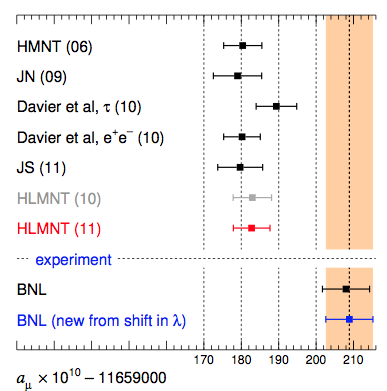
\includegraphics[scale=0.5]{figures/smex}
   \caption[Different SM predictions of $a_{\mu}$]{SM predictions of $a_{\mu}$ calculated by several groups. The new experimental result is due to an improvement in the measurement of the muon-to-proton magnetic moment ratio $\lambda$ \cite{hadlo2}.}
  \label{fig:smex}
\end{figure}

The present error in the SM determination of the anomaly $a_\mu$ is dominated by the errors in the LO VP and LbL contributions, 4.3 $\times 10^{-10}$ and 2.6 $\times 10^{-10}$ respectively. The error in the LO VP is expected to diminish to 2.6 $\times 10^{-10}$ by the expected new data from new collaborations such as VEPP-2000 in Novosibirsk and BES-III at BEPC (China). The projected combined error of LO VP and LbL could go down to 3.0 $\times 10^{-10}$ \cite{new_th}. By combining the proposed Fermilab error of 1.6 $\times 10^{-10}$ with the new expected theoretical error, the total error in the difference between experiment and theory could go down to 3.1 $\times 10^{-11}$, to be compared with the current 7.7 $\times 10^{-11}$. By assuming that the experimental and theoretical values of the anomaly do not change, the new deviation is at the 8.1$\sigma$ level. This last result is an important motivation for the continuous efforts in improving the experimental and theoretical determinations of the muon magnetic moment anomaly.  


\section{Conclusions and Prospects}
\label{fut}
The SM calculation of the anomalous magnetic moment of the muon is smaller than the recent experimental measurement performed by BNL. Depending on the SM evaluation, the discrepancy is approximately $\Delta a_{\mu} \left(\text{E821} - \text{SM}\right) = \left(25.2\pm7.7\right)\times 10^{-10}$, which is larger than the 3$\sigma$ level. This difference will be investigated by a future FNAL experiment which aims at reducing the error in the measurement to 1.6$ \times10^{-10}$. In parallel, theoretical groups aim at reducing the SM error to 3.0 $\times 10^{-10}$.

Currently, candidates such as supersymmetry, extra dimensions, and dark matter models attempt to account for the discrepancy. On the high energy frontier, the LHC is sensitive to the electroweak symmetry breaking (EWSB) scale and its extension that may incorporate new particles and new interactions from the above models. While the first run of the LHC has concluded with the discovery of a new particle compatible with the SM Higgs boson, new physics beyond the SM has not yet been found. The new 2015 run of the LHC is expected to collect a significantly large amount of data at $\sqrt{s}$ = 13 TeV, and thus probe the weak-scale extensions of the SM. However, even if the LHC discovers new effects, it is still not in its capacity to discern between the possible interpretations of different models. In other words, the LHC data might be compatible with different models leading to alternative explanations. For this reason, the LHC requires complementary experiments to determine the properties of any possible new physics. The muon $g-2$ is one of the measurements that is sensitive to parameters not accessible to the LHC. The evaluation of the anomaly is affected by a large class of models describing the TeV scale that may be used to constrain the parameter search at the LHC.

In short, the muon $g-2$ magnetic moment anomaly is sensitive to SM physics and beyond, which is valuable in complementing searches at the LHC, and at the same time constraining existent and future theoretical models. While the discrepancy between experiment and theory has yet to be confirmed with the new FNAL experiment, and more data at higher energy needs to be collected by the LHC to search for new physics, the muon $g-2$ remains an important tool to explore physics beyond the standard model at the TeV scale.

\appendix
\setcounter{chapter}{0}  % Try to change this!!
 
  \chapter{The Dirac Result $\displaystyle g=2$}
 \label{app:dirac}
  \section*{\noindent\small\text{In this section, Gaussian units are used.}}
  
The Dirac equation is a relativistic version of the Schr\"{o}edinger equation written to first order in derivatives which allows a symmetrical treatment of space and time. The derivation follows from the relativistic energy-momentum relation: $\mathcal{E}^2 = (pc)^2+(mc^2)^2$, thus the Hamiltonian can be written as
\[
\mathcal{H} = \left( (cp)^2 + (mc^2)^2 \right)^{1/2}
\]
Dirac found a representation with a set of matrices that satisfies:
\begin{equation}
\label{eq:H}
\mathcal{H} = c \overrightarrow{\gamma}\cdot \overrightarrow{p} + \gamma^0mc^2
\end{equation}
where the $4\times4 \,\,\gamma$ matrices are
\begin{equation}
\begin{split}
\overrightarrow{\gamma} =
\begin{pmatrix}
0 & \overrightarrow{\sigma} \\
\overrightarrow{\sigma} & 0 \\
\end{pmatrix} 
, \,\,\,\,
\gamma^0 =
\begin{pmatrix}
I & 0 \\
0 & -I \\
\end{pmatrix} 
\end{split}
\end{equation}
$I$ is a $2\times2$ identity matrix and $\sigma_i$ for $i=1,2,3$ are the Pauli spin matrices.
By promoting the variables $E$ and $\overrightarrow{p}$ to operators 
\[
\begin{split}
\overrightarrow{p} \to \overrightarrow{P}=-i\hbar\overrightarrow{\nabla},
\,\,\,\,
E \to i\hbar \frac{\partial }{\partial t}
\end{split}
\]
and working in the coordinate basis, the eigenvalue equation $\mathcal{H}  \psi(t) = E \psi(t)$ becomes the Dirac equation:
\begin{equation}
\label{eq:tdse}
i\hbar \frac{\partial \psi(t)}{\partial t} = \left(  c \overrightarrow{\gamma}\cdot \overrightarrow{P} + \gamma^0mc^2  \right) \psi(t)
\end{equation}
where 
\begin{equation}
\label{eq:psit}
\psi(t) = \psi e^{-iEt/\hbar} 
\end{equation}
is a 4-component spinor. Equation (\ref{eq:tdse}) can be written more compactly in the form
\begin{equation}
\left(i\hbar \gamma^{\mu}\partial_{\mu}-\gamma^0mc\right) \psi(t) = 0
\end{equation}
where $\partial_0 =  \frac{1}{c}\frac{\partial}{\partial t}$ and $\partial_i =  \frac{\partial}{\partial x^i}$.

In the presence of a magnetic field represented by a potential $A^{\mu}=(A^0, \overrightarrow{A})$, the Hamiltonian of Equation (\ref{eq:H}) is
\begin{equation}
\label{eq:HB}
\mathcal{H} = c \overrightarrow{\gamma}\cdot \left(\overrightarrow{P}-q\overrightarrow{A}/c\right) + \gamma^0mc^2+qA^0
\end{equation}
and the eigenvalue Equation (\ref{eq:tdse}) becomes
\begin{equation}
\label{eq:eig2}
i\hbar \frac{\partial \psi(t)}{\partial t}  = \left( c\overrightarrow{\gamma}\cdot \overrightarrow{\pi} + \gamma^0mc^2 + qA^0 \right)\psi(t)
\end{equation}
using Equation (\ref{eq:psit}), the result is
\begin{equation}
\label{eq:Epsi}
E \psi = \left( c\overrightarrow{\gamma}\cdot \overrightarrow{\pi} + \gamma^0mc^2 + qA^0 \right)\psi
\end{equation}
where 
\[ \overrightarrow{\pi} =  \overrightarrow{P}-q \overrightarrow{A}/c \]
and $\psi$ is a 4-component object that can be written in terms of two 2-component spinors:
\[
\psi = 
\begin{pmatrix}
\chi \\
\Phi
\end{pmatrix}
\]
Equation (\ref{eq:Epsi}) becomes
\begin{equation}
\label{eq:eig3}
\begin{pmatrix}
E-mc^2-qA^0 & -c\overrightarrow{\sigma}\cdot \overrightarrow{\pi}\\
-c\overrightarrow{\sigma}\cdot \overrightarrow{\pi} & E+mc^2+qA^0
\end{pmatrix}
\begin{pmatrix}
\chi \\
\Phi
\end{pmatrix}
=
\begin{pmatrix}
0 \\
0
\end{pmatrix}
\end{equation}
which leads to
\begin{equation}
\label{eq:cphi}
\left( E-mc^2-qA^0 \right)\chi -c\overrightarrow{\sigma}\cdot \overrightarrow{\pi}\Phi = 0
\end{equation}
\begin{equation}
\left(E+mc^2+qA^0 \right)\Phi -c\overrightarrow{\sigma}\cdot \overrightarrow{\pi}\chi = 0
\end{equation}
The latter equation gives
\begin{equation}
\Phi = \left(\frac{c\overrightarrow{\sigma}\cdot \overrightarrow{\pi}}{ E+mc^2+qA^0 }\right) \chi,
\end{equation}
by working at low velocities, $E + mc^2 \approx 2mc^2$, and at small field-interaction energies compared to the rest mass, $qA^0 < mc^2$, the result is
\begin{equation}
\begin{split}
\Phi &\approx \left(\frac{\overrightarrow{\sigma}\cdot \overrightarrow{\pi}}{ 2mc+qA^0/c }\right) \chi\\
& \approx \frac{1}{2mc} \left( \overrightarrow{\sigma}\cdot \overrightarrow{\pi} \right) \left( 1-\frac{qA^0}{2mc}  \right) \chi
\end{split}
\end{equation}
Plugging this result in Equation (\ref{eq:cphi}), the new equation is 
\begin{equation}
E' \chi = \left\{\frac{1}{2mc} \left( \overrightarrow{\sigma}\cdot \overrightarrow{\pi} \right) \left( \overrightarrow{\sigma}\cdot \overrightarrow{\pi} \right)
\left( 1-\frac{qA^0}{2mc}  \right) + qA^0 \right\}\chi
\end{equation}
where $E' = E-mc^2$. By using the identity
\[\left( \overrightarrow{\sigma}\cdot \overrightarrow{\alpha} \right) \left( \overrightarrow{\sigma}\cdot \overrightarrow{\beta} \right)
=\overrightarrow{\alpha}\cdot \overrightarrow{\beta} + i \overrightarrow{\sigma}\cdot \overrightarrow{\alpha}\times \overrightarrow{\beta}
\]
and 
\[\overrightarrow{\pi}\times \overrightarrow{\pi} = \frac{iq\hbar}{c} \overrightarrow{B}
\]
which can be derived by letting the left hand side act on a spinor $\phi$, using the definition of $\overrightarrow{\pi}$ along with the derivative rule of a product, and recalling that 
$\overrightarrow{\nabla} \times \overrightarrow{A} = \overrightarrow{B}$. The result is
\begin{equation}
\label{eq:dirac_f}
\left\{\frac{\left( \overrightarrow{P}-q \overrightarrow{A}/c \right)^2}{2m} - \frac{q\hbar}{2mc} \overrightarrow{\sigma} \cdot \overrightarrow{B} + qA^0 \right\} \chi = E' \chi,
\end{equation}
the Hamiltonian is then 
\begin{equation}
\label{eq:H_f}
\mathcal{H} = \frac{\left( \overrightarrow{P}-q \overrightarrow{A}/c \right)^2}{2m} - \frac{q\hbar}{2mc} \overrightarrow{\sigma} \cdot \overrightarrow{B} + qA^0 
\end{equation}
Since the interaction term between the spin magnetic moment and the magnetic field is 
\begin{equation}
\label{eq:H_int}
\mathcal{H}_{int} = - \overrightarrow{\mu} \cdot \overrightarrow{B} = -g\frac{q\hbar}{2mc}\frac{\overrightarrow{\sigma}}{2}\cdot \overrightarrow{B} 
\end{equation}
Comparing Equation (\ref{eq:H_f}) to Equation (\ref{eq:H_int}) leads to 
\begin{equation}
g = 2.
\end{equation}

\noindent{The above derivation follows Sections 20.1 and 20.2 of \cite{shankar}.}

 \chapter{Spin Dynamics}
  \label{app:bmt}
  \section*{\small{In this section, Gaussian units are used.}}

In an inertial reference frame, the rate of change of a vector in a rotating frame is given by: 

\begin{equation}
\label{eq:ds}
\left(\frac{d \overrightarrow{S}}{d\tau}\right)_{NRF} = \left(\frac{d \overrightarrow{S}}{d\tau}\right)_{RF} + \overrightarrow{\omega}_T \times \overrightarrow{S}
\end{equation}
NRF: Non-Rotating Frame\\
RF: Rotating Frame

In this case the vector $\overrightarrow{S}$ represents the expectation value of the spin operator of a charged elementary particle such as the muon. The Thomas precessional frequency $\overrightarrow{\omega})T$ is due to the acceleration experienced by the muon as it moves under the action 
of external forces in the transverse direction relative to its velocity vector. 

In the muon rest frame, 
\begin{equation}
\label{eq:dsrf}
\left(\frac{d \overrightarrow{S}}{d\tau}\right)_{RF} = \overrightarrow{\mu} \times \overrightarrow{B}_{RF}
\end{equation}
where $\overrightarrow{\mu}$ is the magnetic moment vector, and $\overrightarrow{B}_{RF}$ is the magnetic field seen by the muons at rest. The spin magnetic moment is:
\begin{equation}
\overrightarrow{\mu} = g\frac{e}{2mc}\overrightarrow{S}
\end{equation}
In the laboratory frame, the magnetic field ($\overrightarrow{B}$) and the electric field ($\overrightarrow{E}$) experienced by the muons are related by: 
\begin{equation}
\label{eq:B}
\overrightarrow{B}_{RF} = \gamma \left(\overrightarrow{B}-\overrightarrow{\beta}\times\overrightarrow{E} \right) 
- \frac{\gamma^2}{\gamma+1}\overrightarrow{\beta}\left(\overrightarrow{\beta} \cdot \overrightarrow{B}\right)
\end{equation}
%To first order in $\overrightarrow{\beta}$, $\gamma \to 1$: 
%\begin{equation}
%\overrightarrow{B}_{RF} = \overrightarrow{B}-\overrightarrow{\beta}\times\overrightarrow{E} 
%\end{equation}
Equation (\ref{eq:dsrf}) becomes:
\begin{equation}
\label{eq:dsrf2}
\left(\frac{d \overrightarrow{S}}{d\tau}\right)_{RF} = g\frac{e}{2mc}\overrightarrow{S} \times \{\gamma \left(\overrightarrow{B}-\overrightarrow{\beta}\times\overrightarrow{E} \right)
- \frac{\gamma^2}{\gamma+1}\overrightarrow{\beta}\left(\overrightarrow{\beta} \cdot \overrightarrow{B}\right)\}
\end{equation}


In order to determine $\overrightarrow{\omega}_T$, consider a system undergoing a sidewise acceleration where the rest frame of this system is different at every instant. The spin direction in the 
laboratory frame is constantly changing even in the absence of torque. By finding the connection between the coordinates in the muon's rest frame and the coordinates in the laboratory frame, 
the rate of change of the spin vector can be determined. At time $t$, the muon rest frame ($x$) is moving with velocity $\overrightarrow{v} = \overrightarrow{\beta}c$ with respect to the laboratory frame. The 
two frames can be related by 
\begin{equation}
x' = \mathcal{A}_{boost}\left(\overrightarrow{\beta}\right)x
\end{equation}
At time $t+\delta t$, the rest frame is moving with a velocity $\overrightarrow{\beta} + \delta \overrightarrow{\beta}$, thus:  
\begin{equation}
x'' = \mathcal{A}_{boost}\left(\overrightarrow{\beta} +  \delta\overrightarrow{\beta}\right)x
\end{equation}
The relation between the two instantaneous rest frames at times $t$ and $t+\delta t$ is: 
\begin{equation}
x'' = \mathcal{A}_{boost}\left(\overrightarrow{\beta} +  \delta \overrightarrow{\beta}\right)\mathcal{A}_{boost}\left(-\overrightarrow{\beta}\right)x'
\end{equation}
The vector quantities of interest are:
 \[
\overrightarrow{\beta} = \left(\beta, 0, 0  \right)
\]
\[
\delta \overrightarrow{\beta} = \left(\delta \beta_1, \delta \beta_2, 0  \right)
\]
\[
\overrightarrow{\beta} + \delta \overrightarrow{\beta} = \left(\beta + \delta \beta_1, \delta \beta_2, 0    \right)
\]

At time $t$, the boost is 
\[
\mathcal{A}_{boost}\left(-\overrightarrow{\beta}\right) =
\begin{pmatrix}
\gamma & \gamma \beta & 0 & 0 \\
\gamma \beta & \gamma & 0 & 0 \\
0 & 0 & 1 & 0 \\
0 & 0 & 0 & 1 \\
\end{pmatrix}
\]

and the Lorentz factor is 
\[
\gamma = \left(1-\beta^2 \right)^{-1/2},
\]
At time $t + \delta t$, the Lorentz factor becomes 
\[
\gamma' = \left(1-\left(\overrightarrow{\beta} +  \delta \overrightarrow{\beta} \right)^2 \right)^{-1/2}. 
\]
To first order, 
\[
\gamma' = \gamma + \gamma^3\beta \delta \beta_1, 
\]
and the boost is 
\[
\mathcal{A}_{boost}\left(\overrightarrow{\beta} +  \delta \overrightarrow{\beta}  \right) =
\begin{pmatrix}
\gamma + \gamma^3\beta \delta \beta_1 & -\left(\gamma \beta + \gamma^3 \delta \beta_1\right) & -\gamma \beta_2 & 0 \\
-\left(\gamma \beta + \gamma^3 \delta \beta_1\right)   & \gamma + \gamma^3\beta \delta \beta_1 & \left(\frac{\gamma-1}{\beta} \right) \delta \beta_2 & 0 \\
-\gamma \beta_2 & \left(\frac{\gamma-1}{\beta} \right) \delta \beta_2  & 1 & 0 \\
0 & 0 & 0 & 1 \\
\end{pmatrix}
\]
(see Equation (11.98) of \cite{jackson}). So
\[
\mathcal{A}_{boost}\left(\overrightarrow{\beta} +  \delta \overrightarrow{\beta}  \right) \mathcal{A}_{boost}\left(-\overrightarrow{\beta}\right) =
\begin{pmatrix}
1 & -\gamma^2 \delta \beta_1 & -\gamma \delta \beta_2 & 0 \\
-\gamma^2 \delta \beta_1 & 1 & \left(\frac{\gamma-1}{\beta} \right) \delta \beta_2 & 0 \\
-\gamma \delta \beta_2 & - \left(\frac{\gamma-1}{\beta} \right) \delta \beta_2 & 1 & 0 \\
0 & 0 & 0 & 1\\
\end{pmatrix}
\]
Define $\mathcal{A}_T$ such that 
\[
\mathcal{A}_T \equiv \mathcal{A}_{boost}\left(\overrightarrow{\beta} +  \delta \overrightarrow{\beta}  \right) \mathcal{A}_{boost}\left(-\overrightarrow{\beta}\right) =
1 + \frac{\gamma - 1}{\beta} \delta \beta_2 S_3 - \gamma^2 \delta \beta_1 K_1 - \gamma \delta \beta_2 K_2
\]
where \\
$
S_3 = 
\begin{pmatrix}
0 & 0 & 0 & 0\\
0 & 0 & -1 & 0\\
0 & 1 & 0 & 0\\
0 & 0 &0 & 0\\
\end{pmatrix},
$  
$
K_1 = 
\begin{pmatrix}
  0 & 1 &0 & 0\\
1 & 0 & 0 & 0\\
0 & 0 & 0 & 0\\
0 & 0 &0 & 0\\
\end{pmatrix},
$
$
K_2 =
\begin{pmatrix}
0 & 0 & 1 & 0\\
0 & 0 & 0 & 0\\
1 & 0 & 0 & 0\\
0 & 0 &0 & 0\\
\end{pmatrix}
$\\\\ (See Section 11.7 of \cite{jackson}).

\[
\mathcal{A}_T = 1- \frac{\gamma - 1}{\beta^2}\left(\overrightarrow{\beta}\times \delta \overrightarrow{\beta}\right)\cdot \overrightarrow{S} - \left(\gamma^2 \delta \overrightarrow{\beta}_{\parallel}
+ \gamma \delta \overrightarrow{\beta}_{\perp}   \right)\cdot \overrightarrow{K}
\]
In the Lorentz group, $\overrightarrow{S}$ is a $4\times 4$ matrix that generates rotations in a three dimensional space, and $\overrightarrow{K}$ is a $4\times 4$ matrix that produces boosts where
\[
\mathcal{R}_{rotation}\left(\Delta \overrightarrow{\Omega} \right) = e^{-\Delta \overrightarrow{\Omega} \cdot \overrightarrow{S}} \approx I - \Delta \overrightarrow{\Omega} \cdot \overrightarrow{S}
\]
\[
\mathcal{A}_{boost}\left(\Delta \overrightarrow{\beta} \right) = e^{-\Delta \overrightarrow{\beta} \cdot \overrightarrow{K}} \approx I - \Delta \overrightarrow{\beta} \cdot \overrightarrow{K}
\]
such that 
\[
\Delta \overrightarrow{\beta} = \gamma^2 \delta \overrightarrow{\beta}_{\parallel} + \gamma \overrightarrow{\beta}_{\perp} 
\]
\[
\Delta \overrightarrow{\Omega} =\frac{\gamma^2}{\gamma + 1} \overrightarrow{\beta} \times \delta\overrightarrow{\beta}.
\]
Again to first order in $\delta\overrightarrow{\beta}$: 
\[
\mathcal{A}_T = \mathcal{A}_{boost}\left(\Delta \overrightarrow{\beta} \right) \cdot \mathcal{R}_{rotation}\left(\Delta \overrightarrow{\Omega} \right)
\]
The transformation from the reference frame at time $t$, $x'$, to a reference frame at time $t+\delta t$, $x''$, introduces an angular change $\Delta \Omega$ which varies at a rate:
\[
\overrightarrow{\omega} = - \lim_{\delta t \to 0} \frac{\Delta \overrightarrow{\Omega}}{\delta t} = -\frac{\gamma^2}{\gamma + 1} \overrightarrow{\beta} \times \frac{d\overrightarrow{\beta}}{dt}
\] 
This relation is the Thomas angular frequency:
\begin{equation}
\label{eq:wt}
\overrightarrow{\omega}_T = \frac{\gamma^2}{\gamma + 1} \frac{\overrightarrow{a}\times \overrightarrow{v}}{c^2}
\end{equation}

By substituting Equation (\ref{eq:wt}) into Equation (\ref{eq:ds}), the new expression for the rate of change of the spin vector is:
\begin{equation}
\label{eq:wt2}
\left(\frac{d \overrightarrow{S}}{d\tau}\right)_{NRF} = \left(\frac{d \overrightarrow{S}}{d\tau}\right)_{RF} + \frac{\gamma^2}{\gamma + 1} \overrightarrow{S} \times 
\left( \overrightarrow{\beta} \times \frac{d \overrightarrow{\beta}}{d\tau} \right)
\end{equation}
The time elapsed in the laboratory frame $dt$ is related to the time elapsed in the muon rest frame $d \tau$ by 
\begin{equation}
\label{eq:dt}
d \tau = \frac{dt}{\gamma}
\end{equation}
By using Equations (\ref{eq:dsrf2}), (\ref{eq:wt2}), and (\ref{eq:dt}), the rate of change of the spin vector is thus given by 
\begin{equation}
\label{eq:wt3}
\frac{d \overrightarrow{S}}{dt} = g\frac{e}{2mc}\overrightarrow{S} \times \left\{\overrightarrow{B}-\overrightarrow{\beta}\times\overrightarrow{E}
- \frac{\gamma}{\gamma+1}\overrightarrow{\beta}\left(\overrightarrow{\beta} \cdot \overrightarrow{B}\right)\right\}
+ \frac{\gamma^2}{\gamma + 1} \overrightarrow{S} \times
\left( \overrightarrow{\beta} \times \frac{d \overrightarrow{\beta}}{dt} \right)
\end{equation}

Since the Lorentz force 4-vector is 
\[
\frac{d U^{\alpha}}{d\tau} = \frac{q}{mc}F^{\alpha \beta}U_{\beta}
\]
where $U^{\alpha}$ is the 4-velocity and $F^{\alpha \beta}$ is the field strength tensor, leading to
\[
\frac{d \gamma}{dt} = \frac{q}{mc}\overrightarrow{E}\cdot\overrightarrow{\beta}
\]
\[
\frac{d \left(\gamma \beta\right)}{dt} = \frac{q}{\gamma mc}\{\overrightarrow{E} + \overrightarrow{\beta}\times\overrightarrow{B}\}
\]
which leads to 
\begin{equation}
\label{eq:dbeta}
\frac{d\overrightarrow{\beta}}{dt} = \frac{q}{\gamma mc}\{ \overrightarrow{E} + \overrightarrow{\beta}\times\overrightarrow{B}-\overrightarrow{\beta}\left(\overrightarrow{E}\cdot
\overrightarrow{\beta} \right)  \} 
\end{equation}
From Equations (\ref{eq:wt3}) and (\ref{eq:dbeta}), the result is 
\begin{equation}
\label{eq:dsf}
\frac{d \overrightarrow{S}}{dt} = \frac{q}{mc}\overrightarrow{S} \times \left\{\left(\frac{g}{2}-1 +\frac{1}{\gamma} \right)\overrightarrow{B}
-\left(\frac{g}{2}-1\right) \left(\frac{\gamma}{\gamma+1}\right)\left(\overrightarrow{\beta} \cdot \overrightarrow{B}\right)\overrightarrow{\beta}
+\left(\frac{g}{2}-1+\frac{1}{\gamma+1}\right)\overrightarrow{E}\times\overrightarrow{\beta}
\right\}
\end{equation}
This equation was derived in 1959 by V. Bargmann, L. Michel, and V.L Telegdi and it is known as the BMT equation. Since 
$\displaystyle
\frac{d \overrightarrow{S}}{dt} = \overrightarrow{S} \times \overrightarrow{\omega_s}
$
and $\displaystyle a = \frac{g}{2}-1$, the final result for the spin angular frequency for muons is Equation (\ref{eq:bmtS})
\begin{equation}
\label{eq:wbmt}
\overrightarrow{\omega_s} =  \frac{q}{m_{\mu}c}\left\{\left(a_{\mu} + \frac{1}{\gamma}\right)\overrightarrow{B}    -   a_{\mu}\left(\frac{\gamma}{\gamma + 1}\right)\left(\overrightarrow{\beta} \cdot \overrightarrow{B}\right)\overrightarrow{\beta}   +   \left(a_{\mu}+\frac{1}{\gamma + 1}\right)\overrightarrow{E} \times\overrightarrow{\beta}                 \right\},
\end{equation}

The equation of motion of the velocity vector in a cyclotron is given by Equation (\ref{eq:dbeta}) which can be written in the form $
\displaystyle \frac{d \overrightarrow{\beta}}{dt} = \overrightarrow{\beta} \times \overrightarrow{\omega}_c$.
By making the assumption that the electric field has no component parallel to the velocity vector ($\overrightarrow{\beta}\cdot\overrightarrow{E}$ = 0), the angular cyclotron frequency for muons is given 
by Equation (\ref{eq:c}): 
\begin{equation}
\overrightarrow{\omega_c} = \frac{q}{\gamma m_{\mu}c}\left\{\overrightarrow{B} + \frac{\gamma^2}{\gamma^2-1} \left(\overrightarrow{E} \times \overrightarrow{\beta}\right)\right\}.
\label{eq:c2}
\end{equation}

\noindent{For more details, check \cite{cern} and Sections 11.8 and 11.11 of \cite{jackson}.}


 \chapter{Muon Decay Rate}
  \label{app:muon}
 \section*{\small{In this section, natural units $c=\hbar=1$ and conventions of \cite{peskin} are used.}}
 
The differential muon decay rate is derived by using the Feynman rules for electroweak processes. The decay
\begin{equation}
\mu\left(p_1\right) \to \nu_{\mu}\left(p_2 \right) + e\left(p_1' \right) + \bar{\nu}_e\left(p_2' \right)
\label{eq:mudecay}
\end{equation}
 is represented by the Feynman diagram
\begin{figure}[H]
  \centering
  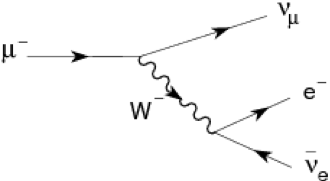
\includegraphics[scale=.5]{figures/FD_muon}
  \label{fig:cp}
\end{figure}
The Amplitude is 
\begin{equation}
\begin{split}
\mathcal{M} = &\int \frac{d^4k}{\left(2\pi\right)^4}\delta^4\left(p_1-p_2-k\right)\bar{u}_2\frac{ig}{2\sqrt{2}}\gamma_{\mu}\left(1-\gamma_5\right)u_1 \frac{-i\left(g^{\mu\nu}-\frac{k^{\mu}k^{\nu}}{m_W^2}
\right)}{k^2-m_W^2+i\epsilon}\times \\& \delta^4\left(k-p_1'-p_2'\right)\bar{u_1}' \frac{ig}{2\sqrt{2}}\gamma_{\nu}\left(1-\gamma_5 \right)v_2'
\label{eq:muM}
\end{split}
\end{equation}
By performing the delta function integral over $k$, canceling the remaining delta function, and using the Dirac equations:
\begin{equation*}
\begin{split}
&\left(\gamma_{\mu}p^{\mu}-m  \right) u = 0 \\
& \bar{u} \left(\gamma_{\mu}p^{\mu}-m  \right)   = 0 \\
&\left(\gamma_{\mu}p^{\mu}+m  \right) v = 0 .
\end{split}
\end{equation*}
The amplitude is then 
\begin{equation}
\begin{split}
\mathcal{M} = &\frac{ig^2}{8\left(\left(p_1-p_2 \right)^2-m_W^2 \right)} \{\bar{u}_2 \gamma_{\mu}\left(1-\gamma_5\right)u_1\bar{u}_1'\gamma^{\mu}\left(1-\gamma_5 \right)v_2'- \\
&  \frac{m_{\mu}m_e}{m_W^2}\bar{u}_2\left(1+\gamma_5\right)u_1\bar{u}_1'\left(1-\gamma_5 \right)v_2'   \}
\label{eq:muM2}
\end{split}
\end{equation}
Since $\frac{m_{\mu}m_e}{m_W^2} \approx 8 \times 10^{-9}$, and assuming that $\left(p_1-p_2 \right)^2 \ll m_W^2$, Equation (\ref{eq:muM2}) becomes
\begin{equation}
\mathcal{M} = -\frac{ig^2}{8m_W^2} \{\bar{u}_2 \gamma_{\mu}\left(1-\gamma_5\right)u_1\bar{u}_1'\gamma^{\mu}\left(1-\gamma_5\right)v_2' \}
\label{eq:muM3}
\end{equation}
The squared amplitude is 
\begin{equation}
|\mathcal{M}|^2 = \frac{g^4}{64m_W^4} \{\bar{u}_2 \gamma_{\mu}\left(1-\gamma_5\right)u_1\bar{u}_1'\gamma^{\mu}\left(1-\gamma_5\right)v_2'\}
\{\bar{v}_2' \gamma_{\nu}\left(1-\gamma_5\right)u_1'\bar{u}_1\gamma^{\nu}\left(1-\gamma_5\right)u_2\}
\label{eq:MM}
\end{equation}
where there is an implicit summation over Dirac indices. By rearranging the previous equation and taking the trace due to the summation, the squared amplitude is
\begin{equation}
|\mathcal{M}|^2 = \frac{g^4}{64m_W^4} Tr[u_2\bar{u}_2 \gamma_{\mu}\left(1-\gamma_5\right)u_1\bar{u}_1\gamma_{\nu}\left(1-\gamma_5\right)]
Tr[u_1'\bar{u}_1'\gamma^{\mu}\left(1-\gamma_5\right)v_2'\bar{v}_2'\gamma^{\nu}\left(1-\gamma_5\right)].
\label{eq:MM}
\end{equation}
By using the spinor combination 
\begin{equation}
u\bar{u} = \left( \gamma_{\mu}p^{\mu} + m \right)\frac{1+\gamma_5\gamma_{\nu}s^{\nu}}{2}
\end{equation}
where $s^{\nu}$ is the spin direction, and using the gamma matrices properties
\begin{itemize}
\item Trace of odd number of gamma matrices is zero.
\item $\left( 1-\gamma_5 \right)^2 = \left( 1-\gamma_5\right)$.
\item $\gamma_5$ anti-commutes with $\gamma_{\mu}$.
\item $\gamma_5\left(1-\gamma_5 \right) = -\left(1-\gamma_5 \right)$.
\end{itemize}
the first trace is
\begin{equation}
\begin{split}
&Tr[u_2\bar{u}_2 \gamma_{\mu}\left(1-\gamma_5\right)u_1\bar{u}_1\gamma_{\nu}\left(1-\gamma_5\right)] = \\
&Tr[\gamma_{\rho}p_2^{\rho}\gamma_{\mu}\left(1-\gamma_5\right)\left(\gamma_{\lambda}p_1^{\lambda} +m_{\mu}\gamma_5\gamma_{\lambda}s_{\mu}^{\lambda} \right)\gamma_{\nu}\left(1-\gamma_5\right)] \\
\end{split}
\end{equation}
where the neutrino masses are negligible. The squared amplitude is then
\begin{equation}
\begin{split}
|\mathcal{M}|^2  = & \frac{g^4}{64 m_W^4} \{p_2^{\rho}\left(p_1^{\lambda}-m_{\mu}s_{\mu}^{\lambda}\right)\left(p_1'^{\alpha}-m_{e}s_{e\alpha}\right)p_{2\beta}'Tr[\gamma_{\rho}\gamma_{\mu}
\gamma_{\lambda}\gamma_{\nu}\left(1-\gamma_5\right) ]  \\
& Tr[\gamma^{\alpha}\gamma^{\mu}\gamma^{\beta}\gamma^{\nu}\left(1-\gamma_5\right)]    \}\\
& = \frac{g^4}{m_W^4}[p_2\cdot\left(p_1'-m_e s_e \right) ] [\left(p_1 - m_{\mu}s_{\mu}\right) \cdot p_2'  ].  
\label{eq:MMM}
\end{split}
\end{equation}
where the identity 
\begin{equation}
\begin{split}
g^{\mu \nu}g^{\alpha \beta} &Tr[\gamma_{\delta}\gamma_{\mu}\gamma_{\phi}\gamma_{\beta}\left(C_1-C_2\gamma_5\right)] 
Tr[\gamma_{\lambda}\gamma_{\nu}\gamma_{\rho}\gamma_{\alpha}\left(C_3-C_4\gamma_5\right)] = \\
&32[C_1C_3\left(\delta_{\delta\lambda}\delta_{\phi\rho}+\delta_{\delta\rho}\delta_{\phi\lambda} \right)
+ C_2 C_4 \left(\delta_{\delta\lambda}\delta_{\phi\rho}-\delta_{\delta\rho}\delta_{\phi\lambda}\right)]
\end{split}
\end{equation}
was used to get the last line in Equation (\ref{eq:MMM}).
The Golden rule relates the differential decay probability of a process with the amplitude squared by the relation:
\begin{equation}
d\Gamma\left(p_1\to p_2p_1'p_2'\right) = \frac{\left(2\pi\right)^4 |\mathcal{M}|^2}{2E_1}\delta^4\left(p_2+p_1'+p_2'-p_1 \right)
\frac{d^3p_2}{\left(2\pi\right)^3 2E_2}\frac{d^3p_1'}{\left(2\pi\right)^3 2E_1'}\frac{d^3p_2'}{\left(2\pi\right)^3 2E_2'}
\end{equation}
Since neutrino momenta are not measured, the integration over the momenta $p_2$ and $p_2'$ is first performed. 
\begin{equation}
\label{eq:dnus}
\begin{split}
d\Gamma\left(p_1\to p_2p_1'p_2'\right) = &\int\frac{d^3p_2}{\left(2\pi\right)^3 2E_2}\frac{d^3p_2'}{\left(2\pi\right)^3 2E_2'}\delta^4\left(p_2+p_1'+p_2'-p_1 \right)p_2^\alpha p_2'^\beta 
\times \\
& \frac{\left(2\pi\right)^4}{2E_1} \frac{g^4}{m_W^4} \left(p_1'-m_e s_e \right)_\alpha \left(p_1 - m_{\mu}s_{\mu}\right)_\beta
\frac{d^3p_1'}{\left(2\pi\right)^3 2E_1'}
\end{split}
\end{equation}
The result of the integration over $p_2$ and $p_2'$ has to be a tensor of second rank with a term $X^\alpha X^\beta$ and a scalar $X^2$ where 
\[X^\alpha = p_1'^\alpha-p_1^\alpha = p_2^\alpha + p_2'^\alpha\]
 \begin{equation}
\label{eq:x2}
X^2 = 2p_2\cdot p_2'
 \end{equation}
 The integral over the neutrino momenta is then 
 \begin{equation}
 \label{eq:int}
 \int\frac{d^3p_2}{ 2E_2}\frac{d^3p_2'}{ 2E_2'}\delta^4\left(X+p_2+p_2' \right)p_2^\alpha p_2'^\beta = Ag^{\alpha\beta}X^2 + B X^\alpha X^\beta
\end{equation}
By doting both sides of Equation (\ref{eq:int}) with $g_{\alpha\beta}$
 \begin{equation}
 \label{eq:int2}
 \int\frac{d^3p_2}{ 2E_2}\frac{d^3p_2'}{ 2E_2'}\delta^4\left(X+p_2+p_2' \right)p_2\cdot p_2' = 4AX^2 + B X^2
\end{equation}
The left hand side contains a standard integral
\[
 \int\frac{d^3b}{ 2b^0}\frac{d^3c}{ 2c^0}\delta^4\left(A-b-c \right) = \frac{\pi \lambda^{1/2}\left(A^2,b^2,c^2 \right)}{2A^2}
\]
where $ \lambda(x,y,z) = x^2+y^2+z^2-2xy-2xz-2yz$. By using Equation (\ref{eq:x2}), the result of the integration is then
\[
\frac{X^2}{2} \frac{\pi}{2} \lambda^{1/2}\left(1,0,0  \right) = 4AX^2 + BX^2
\]
 \begin{equation}
  \label{eq:AB1}
 4A+B = \frac{\pi}{4}
  \end{equation}
 Alternatively, by doting both sides of Equation (\ref{eq:int}) with $X_\alpha X_\beta$, and using
\[
 \left(X-p_2  \right)^2 = 0 = X^2-2X\cdot p_2
 \]
 \[
 \left(X-p_2'  \right)^2 = 0 = X^2-2X\cdot p_2'
 \]
 the result of the integration is
 \[
p_2\cdot X p_2' \cdot X \frac{\pi}{2} \lambda^{1/2}\left(1,0,0  \right) = AX^4 + BX^4
\]
 \begin{equation}
 \label{eq:AB2}
 A+B = \frac{\pi}{8}
  \end{equation}
 From Equation (\ref{eq:AB1}) and Equation (\ref{eq:AB2}): $\displaystyle A = \frac{\pi}{24}$ and $\displaystyle B = \frac{\pi}{12}$. The result of the integral of Equation (\ref{eq:int2}) is 
\begin{equation}
 \int\frac{d^3p_2}{ 2E_2}\frac{d^3p_2'}{ 2E_2'}\delta^4\left(p_1'+p_2+p_2'-p_1 \right)p_2^\alpha p_2'^\beta = \frac{\pi}{24}\left( 
 g^{\alpha\beta}\left(p_1'-p_1\right)^2 + 2 \left(p_1'-p_1\right)^\alpha \left(p_1'-p_1\right)^\beta \right)
 \end{equation}
 Equation (\ref{eq:dnus}) becomes
 \begin{equation}
\label{eq:dnus2}
\begin{split}
d\Gamma= &\frac{g^4d^3p_1'}{192\left(2\pi\right)^4 m_W^4E_1E_1'}
\{\left(p_1'-p_1 \right)^2\left(p_1-m_{\mu} s_{\mu} \right)\cdot\left(p_1'-m_e s_e \right) +\\
& 2\left(p_1'-p_1 \right)\cdot \left(p_1-m_{\mu} s_{\mu} \right)\left(p_1'-p_1 \right)\cdot \left(p_1' - m_e s_e\right)\}
\end{split}
\end{equation}
This equation can be simplified by ignoring the electron mass, choosing a coordinate system in the rest frame of the muon where the angle between the muon spin and the electron momentum is $\theta$, and summing over the final spin states. The result is
 \begin{equation}
\label{eq:dgamma}
\begin{split}
d\Gamma= &\frac{2g^4d^3p_1'}{192\left(2\pi\right)^4 m_W^4 m_\mu E_1'}
\{\left(m_\mu^2-2E_1'm_\mu \right)\left(m_\mu E_1'+m_\mu E_1'\cos \theta \right) +\\
&2\left(m_\mu E_1'-m_\mu^2 + m_\mu E_1'\cos \theta \right)(-m_\mu E_1')\}\\
& = \frac{2g^4E_1'dE_1'd\cos \theta d\phi}{192\left(2\pi\right)^4 m_W^4 m_\mu}\{3m_\mu^3E_1' - 4m_\mu^2 E_1'^2 - m_\mu^3 E_1' \cos \theta +4 m_\mu^2 E_1'^2 \cos \theta \}
\end{split}
\end{equation}
By defining $y = \frac{E_1'}{m_\mu /2}$, Equation (\ref{eq:dgamma}) is
 \begin{equation}
\label{eq:dgamma_f}
\begin{split}
d\Gamma & = \frac{2g^4y^2 dy d\cos \theta d\phi}{192\times 16 \pi^4 m_W^4}\frac{m_\mu^5}{8}
\{3-2y-\cos \theta + 2y \cos \theta\}\\
& = \frac{g^4}{32m_W^2} \frac{ dy d\cos \theta d\phi}{4 \pi} \frac{m_\mu^5}{192 \pi^3}
\{2y^2 \left(3-2y\right)\}\{1+\frac{1-2y}{3-2y}\cos \theta \}
\end{split}
\end{equation}
 This is equivalent to Equation (\ref{eq:prob}) and Equation (\ref{eq:na}).

 
  \chapter{The Schwinger Term $\displaystyle \frac{\alpha}{2\pi}$ }
     \label{app:schwinger}
   \section*{\small{In this section, natural units $c=\hbar=1$ and conventions of \cite{peskin} are used.}}
  


 The QED vertex of the Feynman diagram  
 \begin{figure}[H]
  \centering
  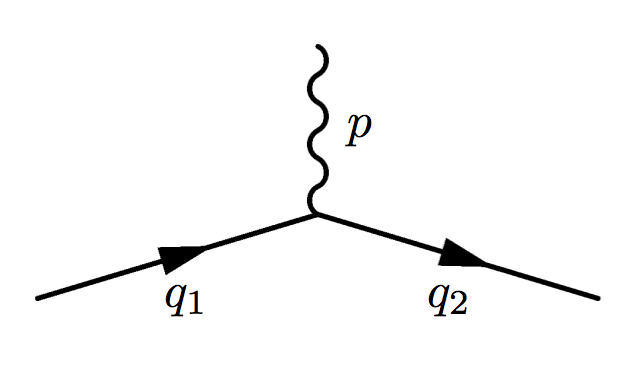
\includegraphics[scale=.2]{figures/qed1}
\end{figure}
is $-ie\gamma^{\mu}$. By analogy, the vertex of the Feynman diagram 
 \begin{figure}[H]
  \centering
  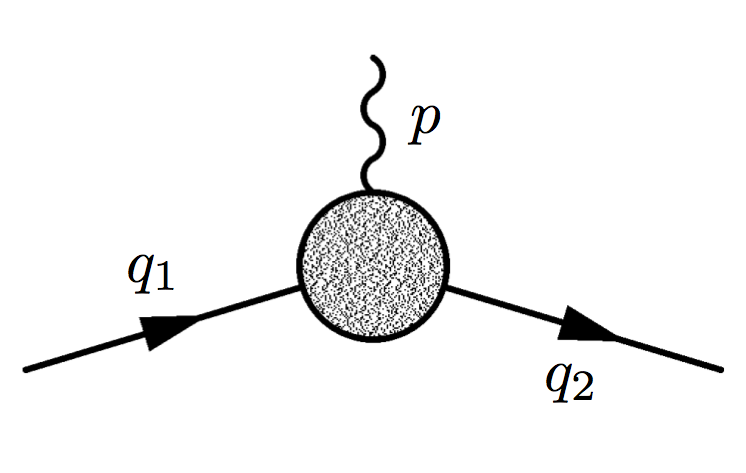
\includegraphics[scale=.2]{figures/qed2}
\end{figure}
is $-ie\Gamma^{\mu}(p_1,p_2)$ where $\Gamma^{\mu}$ is a 4-vector proportional to $\gamma^{\mu}$, $p_1^{\mu}$, and $p_2^{\mu}$. So 
  \begin{equation}
 \Gamma^{\mu} = A\gamma^{\mu}+B(q_1^{\mu}+q_2^{\mu})+C(q_1^{\mu}-q_2^{\mu})
  \end{equation}
where $A$, $B$, and $C$ may be functions of $q_1^2 = q_2^2 = m^2$ and $(q_2-q_1)^2 = p^2$. The use of the Ward identity 
\[\bar{u}(q_2)p_{\mu}\Gamma^{\mu}u(q_1) = 0,\]
and the momentum conservation relation $p^{\mu} = q_2^{\mu} - q_1^{\mu}$ leads to 
\[
\bar{u}(q_2) \{A\left( \cancel{q}_2 - \cancel{q}_1 \right) + B\left(q_2-q_1\right)_{\mu}\left( q_1+q_2 \right)^{\mu} + C \left(q_2-q_1\right)^2\}u(q_1)=0.
 \]
The Dirac equations $\cancel{q}_1u(q_1) = m u(q_1)$ and $ \bar{u}(q_2) \cancel{q}_2 = m \bar{u}(q_2)$, lead to 
\[
\bar{u}(q_2)\left(\cancel{q}_2 - \cancel{q}_1 \right) u(q_1) = \bar{u}(q_2)\left( m-m \right) u(q_1) =0, 
\]
and consequently $C = 0$. Now, by using the Gordon identity of Problem 3.2 of \cite{peskin}
\begin{equation}
\label{eq:gordon}
\bar{u}(q_2) \gamma^{\mu} u(q_1) = \bar{u}(q_2) \{    \frac{q_1^{\mu}+q_2^{\mu}}{2m} + i \frac{\sigma^{\mu\nu}q_{\nu}}{2m} u(q_1) \}
\end{equation}
where $\sigma^{\mu\nu} = \frac{i}{2} [\gamma_{\mu}  ,  \gamma_{\nu} ]$, the $\left(q_1^{\mu}+q_2^{\mu}\right)$ term is eliminated. Rewriting the above expression
 \begin{equation}
 \label{eq:F1F2}
 \Gamma^{\mu}(q_1,q_2) = \gamma^{\mu} F_1 \left( p^2 \right) + \frac{i\sigma^{\mu\nu}p_{\nu}}{2m}F_2\left( p^2 \right),
  \end{equation}
where $F_1$ and $F_2$ are form factors that represent a parametrization of all orders in perturbation theory. In principle, these form factors completely characterize the interaction between the charged lepton, in this case the muon, and the electromagnetic field. %Since the interest is in the magnetic moment coupling, consider a classical static vector potential such that $A_{\mu}^{cl}(x) = \left(0, \overrightarrow{A}_{\mu}^{cl}( \overrightarrow{x}) \right). 
The number of loops in a Feynman diagram determines the order of the contribution, for instance a one loop diagram is of order $\alpha$ and so on. The factor that modifies the muon magnetic moment is $F_2$ at a scale associated with the $p^2$. The first diagram with a single QED vertex is the leading order graph where $F_1 = 1$ and $F_2 = 0$, where in this case $g=2$. By considering higher order contributions, the g factor is $g \to 2 + 2F_2\left(p^2\right)$. For non-relativistic energies 
\begin{equation}
g = 2 + 2F_2(0).
\end{equation}
In order to find the first order correction, $F_2(0)$ should be determined.

According to the Feynman rules, the amplitude of the Feynman diagram 
 \begin{figure}[H]
  \centering
  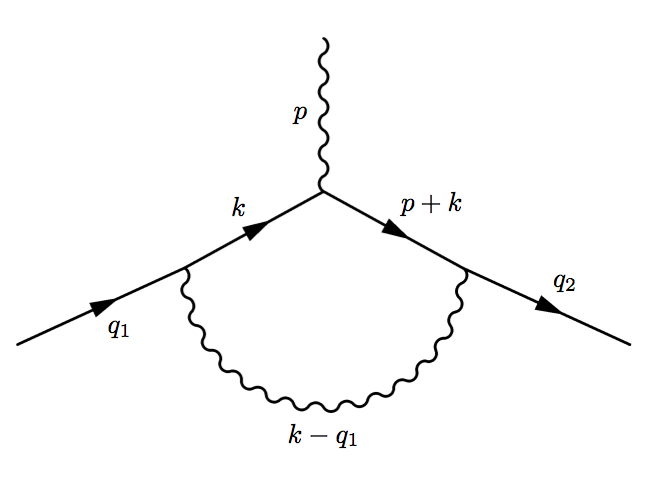
\includegraphics[scale=.35]{figures/qed3}
\end{figure}
is 
 \begin{equation}
 \begin{split}
 i \mathcal{M}^{\mu} = & (-ie)^3\int \frac{d^4k}{(2\pi)^4}\frac{-ig^{\nu\alpha}}{\left( k-q_1 \right)^2+i\epsilon}\bar{u}(q_2)\gamma^{\nu}\frac{i\left(\cancel p + \cancel k + m \right)}{\left(  p+k\right)^2-m^2+i\epsilon}\gamma^{\mu}
 \frac{i\left(\cancel k + m \right)}{  k^2-m^2+i\epsilon}\gamma^{\alpha}u(q_1)\\
 & = -e^3 \bar{u}(q_2) \int \frac{d^4k}{(2\pi)^4}\frac{\gamma^{\nu} \left(\cancel p + \cancel k + m  \right) \gamma^{\mu} \left( \cancel k + m \right) \gamma_{\nu}}
 { \{\left( k-q_1\right)^2+i\epsilon\}\{\left(p+k \right)^2-m^2+i\epsilon\}\{k^2-m^2+i\epsilon\} }u(q_1)
  \end{split}
  \end{equation}
First, the denominator can be simplified according to the relation 
\[
\frac{1}{ABC} = 2 \int_0^1 dx dy dz \delta\left(x+y+z-1\right) \frac{1}{\{xA+yB+zC\}^3}\]
where 
\[
 \begin{split}
 & A = k^2-m^2+i\epsilon\\
& B = \left( p+k\right)^2-m^2+i\epsilon\\
& C = \left( k-q_1 \right)^2 + i\epsilon
 \end{split}.
\]
So the denominator yields
\[
 \begin{split}
\{xA+yB+zC\}^3 &= \{ k^2 + 2k\left(yp-zq_1\right)+yp^2+zq_1^2-\left( x+y\right)m^2+i\epsilon \}^3\\
& = \{ \left(  k^{\mu}+yp^{\mu} - zq_1^{\mu}\right)^2-\Delta +i\epsilon  \}^3
 \end{split}
\]
 where $\Delta = -xyp^2 + \left( 1-z\right)^2m^2$. This expression can be simplified by a change of variables $k^{\mu} \to k^{\mu} -yp^{\mu} + zq_1^{\mu}$ so that the denominator becomes $\left( k^2-\Delta \right)^3$.
 For the numerator ($N^{\mu}$)
 \[
 \begin{split}
N^{\mu} & =   \bar{u}(q_2) \gamma^{\nu}\left(\cancel p + \cancel k + m  \right)\gamma^{\mu}\left( \cancel k + m \right)\gamma_{\nu}u(q_1) \\
& = - 2 \bar{u}(q_2) \{ \cancel k \gamma^{\mu}\cancel p + \cancel k \gamma^{\mu}\cancel k + m^2 \gamma^{\mu}-2m\left( 2k^{\mu}+p^{\mu}\right) \}u(q_1)
\end{split}
 \]
 and by applying the same change in variables, the result is
 \[
  \begin{split}
N^{\mu} = -2\bar{u}(q_2)\{  \left( \cancel k - y \cancel p + z \cancel q_1 \right) \gamma^{\mu}\cancel p + \left( \cancel k - y\cancel p + z \cancel q_1\right) \gamma^{\mu} \left(\cancel k - y \cancel p + z \cancel q_1 \right) \} u(q_1)\\
 +\bar{u}(q_2)\{m^2 \gamma^{\mu} - 2m\left( 2k^{\mu}-2yp^{\mu}+2zq_1^{\mu}+p^{\mu} \right)\}u(q_1)
  \end{split}
 \]
The delta function $\delta\left( x+y+z-1\right)$ implies that $x+y+z=1$, and since $g^{\mu\nu}g_{\mu\nu}=4$, then  $k^{\mu}k^{\nu} = \frac{1}{4}g^{\mu\nu}k^2$, 
the numerator is now
\begin{equation}
\label{eq:N}
\begin{split}
-\frac{1}{2}N^{\mu} = &\left\{ -\frac{1}{2}k^2 + \left(1-x\right)\left(1-y\right)p^2 + \left(1-4z+z^2  \right)m^2 \right\} \bar{u}(q_2)\gamma^{\mu}u(q_1) \\
& + imz\left( 1-z \right)p_{\nu}\bar{u}(q_2)\sigma^{\mu\nu}u(q_1) \\
& +m\left( z-2\right)\left( x-y\right)p^{\mu}\bar{u}(q_2)u(q_1)
\end{split}
\end{equation}
In order to get the magnetic moment contribution, the only term that needs to be considered is the one containing $\sigma^{\mu\nu}$, thus 
\begin{equation}
\label{eq:MM}
i\mathcal{M}^{\mu} = p_\nu\bar u (q_2) \sigma ^{\mu\nu}u(q_1) \left\{ 4ie^3m\int_0^1 dxdydz\delta(x+y+z-1) \int\frac{d^4k}{\left( 2\pi\right)^4} \frac{z\left(1-z\right)}{\left( k^2-\Delta +i\epsilon\right)^3}\right\} + \cdots
\end{equation}
By comparing Equations (\ref{eq:F1F2}) and (\ref{eq:MM}), the form factor $F_2$ is
\begin{equation}
\label{eq:F2}
F_2\left( p^2\right) = \frac{2m}{e}\left( 4ie^3m\right)\int_0^1 dx dy dz\delta(x+y+z-1) \int\frac{d^4k}{\left( 2\pi\right)^4} \frac{z\left(1-z\right)}{\left( k^2-\Delta +i\epsilon\right)^3} + \cdots
\end{equation}
This is a correction to the order $e^2 = \alpha$.
To compute this integral, use  
\begin{equation}
\label{eq:d4k}
\int \frac{d^4k}{\left( 2\pi \right)^4}\frac{1}{\left(k^2-\Delta + i \epsilon \right)^3} = \frac{-i}{32 \pi^2 \Delta}
\end{equation}
(see A.4 of \cite{peskin}). The result of the integral in Equation (\ref{eq:F2}) is then 
\begin{equation}
\label{eq:F22}
F_2\left( p^2 \right) = \frac{\alpha}{\pi}m^2 \int_0^1 dx dy dz\delta(x+y+z-1)\frac{z\left(1-z\right)}{\left(1-z\right)^2m^2-xyp^2}
\end{equation}
Since this integral needs to be evaluated for $p^2 = 0$, the steps follow
\begin{equation}
\label{eq:F20}
\begin{split}
F_2\left( 0 \right) & = \frac{\alpha}{\pi}\int_0^1 dz  \int_0^1 dy \int_0^1 dx \delta(x+y+z-1)\frac{z}{\left(1-z\right)}\\
& =  \frac{\alpha}{\pi} \int_0^1 dz  \int_0^{1-z} dy \frac{z}{1-z}\\
& = \frac{\alpha}{2\pi}
\end{split}
\end{equation}
This result is called the Schwinger term which represents the first order QED correction and by far the largest radiative correction given in Equation (\ref{eq:schwinger}). So to first order in $\alpha$
\begin{equation}
g = 2\left( 1+ \frac{\alpha}{2\pi} \right)
\end{equation}
which agrees with Equation (\ref{eq:schwinger2}). 

\noindent{More details can be found in Sections 6.2 and 6.3 of \cite{peskin}.}

%% You need a file named `g-2_references.bib' to use BibTex here
\bibliography{g-2_references}

% \backmatter

% remarks:
% cyclotron period 149 ns
% muon-to-proton magnetic moment was determined as follow: measurement of the hyperfine interval of ground state muonium $\Delata \nu_{HFS}$ to 12 ppb. The theoretical prediction for the hyperfine interval,  $\Delata \nu_{HFS,th}$ depends on $\mu_{\mu}/\mu_{\p}$, by equating the two, the ratio was determined to 30ppb. this value agrees with value a measurement of two Zeeman hyperfine transitions in muonium in a strong magnetic field to 120 ppb. This means that the absolute calibration probe used to get the fre proton from the precession of the proton in water is good to 120ppb. See p51 BNL

\end{document}


